\documentclass{article}


% if you need to pass options to natbib, use, e.g.:
%     \PassOptionsToPackage{numbers, compress}{natbib}
% before loading neurips_2023


% ready for submission
\usepackage{neurips_2023}
\usepackage{tikz}
\usepackage{pgfplots}
\pgfplotsset{compat=1.18}
\pgfplotsset{
    myplotstyle/.style={
    ylabel style={align=center, font=\bfseries\boldmath},
    xlabel style={align=center, font=\bfseries\boldmath},
    x tick label style={font=\bfseries\boldmath},
    y tick label style={font=\bfseries\boldmath},
    scaled ticks=false,
    every axis plot/.append style={thick},
    xmin = 0 , xmax=100, ymin = 0, ymax = 3,
    },
}
%legend style={draw=none, font=\small},
    %legend cell align=left,
    %legend pos=north east,
\usepackage{amsmath}
% to compile a preprint version, e.g., for submission to arXiv, add add the
% [preprint] option:
%\usepackage[preprint]{neurips_2023}


% to compile a camera-ready version, add the [final] option, e.g.:
%usepackage[final]{neurips_2023}


% to avoid loading the natbib package, add option nonatbib:
%    \usepackage[nonatbib]{neurips_2023}


\usepackage[utf8]{inputenc} % allow utf-8 input
\usepackage[T1]{fontenc}    % use 8-bit T1 fonts
%\usepackage{hyperref}       % hyperlinks
\usepackage{url}            % simple URL typesetting
\usepackage{booktabs}       % professional-quality tables
\usepackage{amsfonts}       % blackboard math symbols
\usepackage{nicefrac}       % compact symbols for 1/2, etc.
\usepackage{microtype}      % microtypography
\usepackage{xcolor}         % colors
\usepackage{epstopdf}
\usepackage{microtype}      % microtypography
\usepackage{xcolor}         % colors
\usepackage{amssymb}
\usepackage{mathtools}
\usepackage{amsthm}
\usepackage{graphicx}
%\usepackage{subfigure}
\usepackage{caption}
\usepackage{subcaption}
\usepackage{algpseudocode,algorithm,algorithmicx}
\newcommand{\hcm}[1]{\textcolor{blue}{#1}}
\theoremstyle{plain}
\newtheorem{theorem}{Theorem}[section]
\newtheorem{proposition}[theorem]{Proposition}
\newtheorem{lemma}[theorem]{Lemma}
\newtheorem{corollary}[theorem]{Corollary}
\theoremstyle{definition}
\newtheorem{definition}[theorem]{Definition}
\newtheorem{assumption}[theorem]{Assumption}
\theoremstyle{remark}
\newtheorem{remark}{Remark}[theorem]
\algrenewcommand\algorithmicrequire{\textbf{Precondition:}}  
\algrenewcommand\algorithmicensure{\textbf{Postcondition:}}
\title{A Variational Perspective on High-Resolution ODEs}


% The \author macro works with any number of authors. There are two commands
% used to separate the names and addresses of multiple authors: \And and \AND.
%
% Using \And between authors leaves it to LaTeX to determine where to break the
% lines. Using \AND forces a line break at that point. So, if LaTeX puts 3 of 4
% authors names on the first line, and the last on the second line, try using
% \AND instead of \And before the third author name.


\author{%
  Hoomaan ~Maskan\thanks{Use footnote for providing further information
    about author (webpage, alternative address)---\emph{not} for acknowledging
    funding agencies.} \\
  Department of Mathematics \& \\Mathematical Statistics\\
  Umeå University\\
  Umeå, Sweden 90736 \\
  \texttt{hoomaan.maskan@umu.se} \\
  % examples of more authors
   %\And
   %Coauthor \\
  % Affiliation \\
  % Address \\
  % \texttt{email} \\
  % \AND
  % Coauthor \\
  % Affiliation \\
  % Address \\
  % \texttt{email} \\
  % \And
  % Coauthor \\
  % Affiliation \\
  % Address \\
  % \texttt{email} \\
  % \And
  % Coauthor \\
  % Affiliation \\
  % Address \\
  % \texttt{email} \\
}


\begin{document}


\maketitle


\begin{abstract}
We consider unconstrained minimization of smooth convex functions. We propose a novel variational perspective using forced Euler-Lagrange equation that allows for studying high-resolution ODEs. Through this, we obtian a faster convergence rate for gradient norm minimization using Nesterov's accelerated gradient method. Additionally, We show that rate-matching discretization technique implicitly perturbs. Furthermore, we propose a stochastic method for noisy gradients. 
\end{abstract}


\section{Introduction}

Optimization algorithms play an important role in big data analysis and machine learning. Due to huge load of data, accelerated methods in optimization are important and necessary to study \citep{Shi2021UnderstandingTA,JMLR:v17:15-084,wilson2021lyapunov,Lessard2016AnalysisAD}. \par
Consider the following unconstrained minimization problem
\begin{align}\label{problem}
    \min_{x\in \mathbb{R}^n} f(x)
\end{align}

where $f:\mathbb{R}^n\rightarrow \mathbb{R}$ and \(f\in\mathcal{F}_{L}\) where \(\mathcal{F}_{L}\) denotes the class of \(L\)-smooth and convex functions on \(\mathbb{R}^n\) i.e.,
\begin{align}\label{cvx-smthness}
 f(x)-f(y)\leq \langle \nabla f(x),x-y \rangle,\quad \|\nabla f(x_k)-\nabla f(y_k)\|\leq L \|x-y\|,
\end{align}
where \(\|\cdot\|\) denotes the Euclidean norm. Nesterov's Accelerated Gradient (NAG) method was among the first accelerated\footnote{Here, acceleration is w.r.t the convergence rate of the Gradient Descent (GD) method.} globally convergent algorithms to solve (\ref{problem}) \citep{Nesterov1983AMF},
 \begin{align}\label{eqn_Nest_alg}
    y_{k+1}&=x_k -s\nabla f(x_k),\\
    x_{k+1}&= y_{k+1}+\frac{k}{k+3} (y_{k+1}-y_{k}),\nonumber
\end{align}
with \(x_0=y_0\in\mathbb R^n\) and \(0< s\leq 1/L\). The NAG method achieves the first order oracle complexity lower bound with a convergence rate of \(f(x_k)-f(x^*)=\mathcal O (1/(sk^2))\) \citep{nesterov2003introductory}. Nesterov used \textit{estimate sequence} technique to prove the convergence of the NAG method. Due to the complexity of this technique, the essence of acceleration remained a mystery. Many have tried to provide a better understanding of momentum-based acceleration (like the one in (\ref{eqn_Nest_alg})) through different perspectives. For example, \citep{JMLR:v17:15-084,shi2019acceleration,Shi2021UnderstandingTA,sanz2021connections}, consider a continuous-time perspective, \citep{Lessard2016AnalysisAD,doi:10.1137/17M1136845} use integral quadratic constraints and control systems with non-linear feedbacks, \citep{muehlebach2019dynamical,muehlebach2022constraints,muehlebach2023accelerated} presents a dynamical perspective, and \citep{attouch2020first,attouch2021convergence} utilize inertial dynamic involving both viscous damping and Hessian-driven damping. 
\paragraph{Continuous-time perspective}Analysing the NAG when \(s\rightarrow 0\), exhibits similar trajectories as Ordinary Differential Equations (ODEs) \citep{JMLR:v17:15-084}. This has inspired many to analyse various ODEs and discretization schemes to understand acceleration phenomenon. \citep{WibisonoE7351,wilson2021lyapunov} showed that the recent ODE is a special case of a family of ODEs which were not confined to Euclidean space. They proved their claim through minimizing the action on a Lagrangian which could capture the properties of (\ref{problem}). This is known as the \textit{variational perspective}. They then discretized their general ODE through \textit{rate-matching} technique. On the same line of work, \citep{Shi2021UnderstandingTA} proposed High-Resolution ODEs (HR-ODEs) (opposed to Low-Resolution ODEs (LR-ODEs) by \citep{JMLR:v17:15-084}) which could follow the NAG's trajectory more accurately than LR-ODEs. The remaining question which is mainly discussed in this work is
\begin{center}
   \textit{Is it possible to explain HR-ODEs through variational perspective? If yes, what benefits does this explanation have?} 
\end{center}
\paragraph{Our contribution} We will positively respond to the first part of the question in Section \ref{section2}. This is done by incorporating external forces while minimizing the action on the Lagrangian. We will show that same force with various damping parameters recovers various HR-ODEs. Our variational analysis leads to a special representation of the NAG method in section \ref{section3} which allows for better convergence rates for gradient norm minimization of the NAG method than \citep{shi2019acceleration}. In Section \ref{section4}, we propose the HR-ODE of the rate-matching technique and show that this technique implicitly perturbs an LR-ODE. Finally, we extend our analysis to practical scenarios by considering noisy gradients in Section \ref{section5}. Specifically, we will show a convergence rate of \(\mathcal O(\log(k)/\sqrt{k})\) for function \(f\in\mathcal{F}_L\) and \(\mathcal{O}(\log(k)/k^{3/4})\) for \(\mathbb E\left[\min_{0\leq i\leq k-1}\|\nabla f(x_i)\|^2 \right]\). Several numerical simulations in Section \ref{sec_numerical} approve and compare our findings with state of the art.

 
\section{External Forces and High-Resolution ODEs}\label{section2}
Consider the Bregman Lagrangian
\begin{align}\label{Lagrangian2}
    \mathcal{L}(X_t,\dot{X}_t,t) =e^{\alpha_t+\gamma_t}\left(\frac{1}{2}\|e^{-\alpha_t}\dot{X}_t\|^2-e^{\beta_t}f(X_t)\right). 
\end{align}
where \(\dot{X}_t\in \mathbb{R}^d\) is the first time-derivative of \(X(t)\) and \(\alpha_t,\beta_t,\gamma_t:\mathbb{T}\rightarrow \mathbb{R}\) are continuously differentiable functions of time and correspond to the weighting of velocity, the potential function and the overall damping. From the variational calculus, define the action on the curves \(\{X_t:t\in \mathbb R\}\) as the functional \(\mathcal{A}(X)=\int_{\mathbb R}\mathcal{L}(X_t,\dot X_t,t)dt \). In absence of external forces, the curve which is a stationary point to the problem of minimizing the action \(\mathcal{A}(X)\), will satisfy the Euler Lagrange equation \({\tfrac{d}{dt}\{  \tfrac{\partial \mathcal{L}}{\partial \dot{X}_t}(X_t,\dot{X}_t,t)  \}=\tfrac{\partial \mathcal{L}}{\partial X}(X_t,\dot{X}_t,t)}\). This was used in \citep{WibisonoE7351,wilson2021lyapunov} to calculate the LR-ODEs for convex and strongly convex functions\footnote{\citep{wilson2021lyapunov}, uses different Lagrangian for strongly convex functions, but the methodology is the same.}. However, if an external force \(F\) (which is not derived from the potential \(f\)) exists, the Euler-Lagrange equation modifies to the forced Euler Lagrange Equation
\begin{align}\label{fEL}
        \frac{d}{dt}\left\{  \frac{\partial \mathcal{L}}{\partial \dot{X}_t}(X_t,\dot{X}_t,t)  \right\}-\frac{\partial \mathcal{L}}{\partial X_t}(X_t,\dot{X}_t,t)=F,
\end{align}
which itself is the result of integration by parts of Lagrange d'Alembert principle \citep{campos2021discrete}. Using the Lagrangian (\ref{Lagrangian2}) we have
\begin{align}\label{Lagrange_par_der}
  &   \frac{\partial \mathcal{L}}{\partial \dot{X}_t}(X_t,\dot{X}_t,t)  =e^{\gamma_t}(e^{-\alpha_t}\dot{X}_t),\quad \frac{\partial \mathcal{L}}{\partial X_t}(X_t,\dot{X}_t,t)= -e^{\gamma_t+\alpha_t+\beta_t}(\nabla f(X_t)).
\end{align}
Substituting (\ref{Lagrange_par_der}) in (\ref{fEL}) gives
\begin{align}\label{HR_general_ODE_F}
    \Ddot{X}_t + (\dot{\gamma}_t-\dot{\alpha}_t)\dot{X}_t+e^{2\alpha_t+\beta_t}\nabla f(X_t) =e^{\alpha_t-\gamma_t} F
\end{align}
In what follows, we will present two different choices of the external force \(F\) for convex and one for strongly convex functions. 
\subsection{Convex Functions}
$\boldsymbol {F = -\sqrt{s}e^{\gamma_t}\frac{d}{dt}[e^{-\alpha_t}\nabla f(X)]}:$ 
    In this case, (\ref{HR_general_ODE_F}) gives
    \begin{align}\label{HR_general_ODE_F_laborde}
    \Ddot{X}_t + (\dot{\gamma}_t-\dot{\alpha}_t)\dot{X}_t+e^{2\alpha_t+\beta_t}\nabla f = -\sqrt{s}e^{\alpha_t}\frac{d}{dt}[e^{-\alpha_t}\nabla f(X_t)].
\end{align}
Following theorem shows the convergence of (\ref{HR_general_ODE_F_laborde}). Note that the proof schemes of the theorems in this section are based on the Lyapunov analysis of their corresponding ODEs. Lyapunov function is widely used in solving ODEs \citep{siegel2019accelerated,shi2019acceleration,attouch2020first,attouch2021convergence}. This non-negative function attains zero only at the solution of the corresponding ODE and decreases along the trajectory of the ODE \citep{khalil2002nonlinear}.For each of the following theorems, we will define a proper Lyapunov function and prove sufficient decrease of the function \(f\) along the corresponding ODE's trajectory.
\begin{theorem}\label{Theorem_ODE_laborde}
Under the ideal scaling conditions $\dot\beta_t\leq e^{\alpha_t}, \dot\gamma_t=e^{\alpha t}$, the dynamic (\ref{HR_general_ODE_F_laborde}) for convex function $f$ will satisfy 
$$f(X_t)-f(x^*)\leq \mathcal{O}(e^{-\beta_t})$$
\end{theorem}

Choosing parameters as
\begin{align}\label{prams_general}
        \alpha_t=\log (n(t)),\quad
    \beta_t=\log (q(t)/n(t)),\quad
    \dot\gamma_t=e^{\alpha_t}=n(t),
\end{align}
in (\ref{HR_general_ODE_F_laborde}) gives
\begin{align}\label{HR_cnts_general_npq_laborde}
\left\{
\begin{array}{l}
     \Ddot{X}_t + (n(t)-\frac{\dot n(t)}{n(t)}+\sqrt{s}\nabla^2 f(X_t))\dot{X}_t+(n(t)q(t)-\sqrt{s} \frac{\dot n(t)}{n(t)})\nabla f(X_t)=0,   \\
    F = -\sqrt{s}e^{\gamma_t}\frac{d}{dt}[e^{-\alpha_t}\nabla f(X)],  
\end{array}\right.
\end{align}
which reduces to 
\begin{align}\label{HR_cnts_general_npq2}
     \Ddot{X}_t + (\frac{p+1}{t}+\sqrt{s}\nabla^2 f(X_t))\dot{X}_t+(Cp^2t^{p-2}+\frac{\sqrt{s}}{t})\nabla f(X_t)=0
\end{align}
by taking $n(t)=\frac{p}{t},q(t)=Cpt^{p-1}$. This is a more general form of the high-resolution ODE found in \citep{pmlr-v108-laborde20a}. 
\begin{remark}
For \(p=2,C=1/4\), (\ref{HR_cnts_general_npq2}) reduces to the NAG method using Explicit Euler (EE) discretization with gradient calculated at an updated point \citep{pmlr-v108-laborde20a}.
\end{remark}

     \( \boldsymbol{F = -\sqrt{s}e^{\gamma_t-\beta_t}\frac{d}{dt}\left[e^{-(\alpha_t-\beta_t)}\nabla f(X_t)\right]}:\)
    In this case, replacing $F$ in (\ref{HR_general_ODE_F}) gives
    \begin{align}\label{HR_general_ODE_F_Shi}
    \Ddot{X}_t + (\dot{\gamma}_t-\dot{\alpha}_t)\dot{X}_t+e^{2\alpha_t+\beta_t}\nabla f = -\sqrt{s}e^{\alpha_t-\beta_t}\frac{d}{dt}[e^{-(\alpha_t-\beta_t)}\nabla f(X_t)],
\end{align}
which has the following convergence result. \begin{theorem}\label{Theorem_ODE_Shi}
Under the modified ideal scaling conditions \(\dot\beta_t\leq e^{\alpha_t}, \dot\gamma_t=e^{\alpha t}, \Ddot{\beta}_t\leq e^{\alpha_t}\dot \beta_t + 2\dot \alpha_t \dot \beta_t\), the dynamic (\ref{HR_general_ODE_F_Shi}) for convex function \(f\) will satisfy 
\[f(X_t)-f(x^*)\leq \mathcal{O}(\frac{1}{e^{\beta_t}+\sqrt{s}e^{-2\alpha_t}\dot \beta_t}),\]
\end{theorem}

As it can be inferred, Theorem \ref{Theorem_ODE_Shi} reveals faster convergence rate than Theorem \ref{Theorem_ODE_laborde} which suggests the superiority of the high-resolution ODE found by \citep{Shi2021UnderstandingTA} to the ODE from \citep{pmlr-v108-laborde20a}. Taking the same parameters (\ref{prams_general}) gives
\begin{gather}
    \begin{aligned}\label{HR_cnts_general_npq_SHI}
\left\{
\begin{array}{l}
     \Ddot{X}_t + (n(t)-\frac{\dot n(t)}{n(t)}+\sqrt{s}\nabla^2 f(X_t))\dot{X}_t+(n(t)q(t)-\sqrt{s} (\frac{\dot n(t)}{n(t)}-\frac{\dot q(t)n(t)-\dot n(t)q(t)}{n(t)q(t)}))\nabla f(X_t)=0,   \\
     F = -\sqrt{s}e^{\gamma_t-\beta_t}\frac{d}{dt}\left[e^{-(\alpha_t-\beta_t)}\nabla f(X_t)\right]. 
\end{array}\right.\raisetag{12pt}
\end{aligned}
\end{gather}
 
which reduces to
\begin{align}\label{HR_cnts_general_npq_p}
     \Ddot{X}_t + (\frac{p+1}{t}+\sqrt{s}\nabla^2 f(X_t))\dot{X}_t+(Cp^2t^{p-2}+\frac{\sqrt{s}(p+1)}{t})\nabla f(X_t)=0,
\end{align}
for \(n(t)=p/t,q(t)=Cpt^{p-1}\). 
\begin{remark}
    Note that setting \(C=1/4,p=2\) will lead to the ODE 
\begin{align}\label{HR_cnts_general_stable_ODE}
     \Ddot{X}_t + (\frac{3}{t}+\sqrt{s}\nabla^2 f(X_t))\dot{X}_t+(1+\frac{3\sqrt{s}}{t})\nabla f(X_t)=0,
\end{align}
which was shown to be accelerated after Semi-Implicit-Euler (SIE) discretization in \citep{shi2019acceleration}.
\end{remark}
\subsection{Strongly Convex Functions:} Our analysis is applicable to strongly convex functions as well. Using the Lagrangian proposed in \citep{wilson2021lyapunov} for strongly convex functions we have
\begin{align}\label{strongly_cvx_lagrange}
    \mathcal{L}(X_t,\dot X_t,t)=e^{\alpha_t+\beta_t+\gamma_t}(\mu \frac{1}{2}\|e^{-\alpha_t}\dot X_t\|^2-f(X_t)).
\end{align}
Then, the forced Euler-Lagrange equation (\ref{fEL}) becomes
\begin{align}\label{HR_FEL}
    \Ddot{X}+(-\dot \alpha_t + \dot 
 \gamma_t+ \dot \beta_t)\dot X+\frac{1}{\mu}e^{2\alpha_t}\nabla f(X)=\frac{F}{\mu e^{-\alpha_t + \gamma_t + \beta_t}}.
\end{align}
\(\boldsymbol{F=-\sqrt{s}e^{\alpha_t+\gamma_t}\frac{d}{dt}(e^{\beta_t}\nabla f(X_t))}\): Replacing in (\ref{HR_FEL}) we get
\begin{align}\label{sc_eqn1}
    \Ddot{X}+(-\dot \alpha_t + \dot 
 \gamma_t+ \dot \beta_t)\dot X+\frac{1}{\mu}e^{2\alpha_t}\nabla f(X)=\frac{-\sqrt{s}e^{2\alpha_t-\beta_t}\frac{d}{dt}(e^{\beta_t}\nabla f(X_t))}{\mu }.
\end{align}
The following theorem shows the convergence of (\ref{sc_eqn1}).
\begin{theorem}\label{Theorem3_1}
    Under the modified ideal scaling conditions \(\alpha_t=\alpha\), \(\dot \beta_t\leq e^{\alpha_t}\), \(\dot \gamma_t=e^{\alpha_t}\), and \(\dot \beta_t\geq 0\) the dynamic (\ref{sc_eqn1}) will satisfy
    \begin{align}\label{Theorem32_eqn1}
      f(X_t)-f(x^*)\leq \mathcal{O}(e^{-\beta_t})  
    \end{align}
    for \(\mu\)-strongly convex function \(f\).
\end{theorem}
\begin{remark}
    Taking \(\alpha=\log(\sqrt{\mu})\) and \(\gamma_t=\beta_t=\sqrt{\mu}t\) in (\ref{sc_eqn1}) gives the high-resolution ODE 
\begin{align}\label{high-res-ODE}
    \Ddot{X}_t+(2\sqrt{\mu}+\sqrt{s}\nabla^2 f(X_t))\dot X_t +(1+\sqrt{\mu s })\nabla f(X_t)=0,
\end{align}
for \(\mu\)-strongly convex function \(f\) as in \citep{Shi2021UnderstandingTA}.
\end{remark}
\section{Gradient Norm Minimization of the NAG}\label{section3}
One of the implications of variational HR-ODEs in Section \ref{section2} was the ODE (\ref{HR_cnts_general_stable_ODE}). Rewriting this ODE gives
\begin{align}\label{Two_oneline_ODE_perturbed}
   \left\{ \begin{array}{ll}
    & \dot{X_t}   =     n(t)(V_t-X_t)-\sqrt{s}\nabla f(X_t)\\
     &\dot{V_t}    =  -q(t)\nabla f(X_t) - \sqrt{s}\frac{\dot q(t)n(t)-\dot n(t)q(t)}{n^2(t)q(t)} \nabla f(X_t).
    \end{array}\right.
\end{align}
Applying SIE on (\ref{Two_oneline_ODE_perturbed}) for \({X(t) \approx X(t_k), V(t)\approx V(t_k),n(t_k)=p/t_k,q(t_k)=Cpt_k^{p-1},}\) 
\({ p=2,t_k=k\sqrt{s}}\) and \(C=1/4\) gives 
\begin{align}\label{new_algorithm}
   \left\{ \begin{array}{ll}
    &x_{k+1}   =    x_{k} + \frac{2}{k}(v_k-x_{k+1})-{s}\nabla f(x_k),\\
     &v_{k+1}    = v_k -\tfrac{1}{2}((k)s)\nabla f(x_{k+1})-s\nabla f(x_{k+1}), 
    \end{array}\right.
\end{align}
 which is exactly the NAG algorithm. The representation (\ref{new_algorithm}) of the NAG algorithm is less investigated in the literature (see \citep{ahn2022understanding} for the four most studied representations). The form of (\ref{new_algorithm}) leads to faster convergence rate for gradient norm minimization of the NAG algorithm than \citep{Shi2021UnderstandingTA}. The following theorem formulates this result. The proof is in Appendix \ref{thm5_proof} and is based on the discrete Lyapunov analysis of (\ref{new_algorithm}). Similar convergence rate was very recently found by \citep{chen2022gradient} (through \textit{implicit velocity} perspective on HR-ODEs which is a totally different approach from this work). This was concurrent to the preparation of this work.
\begin{theorem}\label{theorem4}
    Consider the update (\ref{Two_oneline_ODE_perturbed}) with \(n(t_k)=p/t_k,q(t_k)=Cpt_k^{p-1}\) and \(p=2,t_k=k\sqrt{s},C=1/4\). Then, if \(f\) is convex and \(L\)-smooth we have
    \[\min_{0\leq i\leq k-1}\|\nabla f(x_i)\|^2 \leq \frac{12}{k^3s^2}\|x_0-x^*\|^2,\]
    and
    \[f(x_k)-f(x^*)\leq \frac{2}{sk(k+2)}\|x_0-x^*\|^2\]
    for \(0\leq s\leq 1/L\) and \(x_0=v_0\).
\end{theorem}
\begin{remark}[Comparison with stare of the art]
    The rate in Theorem \ref{theorem4} is improved compared to the previous rate found by \citep{Shi2021UnderstandingTA} which was 
$$ \min_{0\leq i\leq k}\|\nabla f(x_i)\|^2 \leq \frac{8568}{(k+1)^3s^2}\|x_0-x^*\|^2,$$
for $0< s\leq 1/(3L)$ and $k\geq0$.
\end{remark}
\begin{remark}
\citep{shi2019acceleration} did not recover the ODE (\ref{HR_cnts_general_stable_ODE}). In fact, they proposed 
\begin{align}\label{HR_cnts_general_non_stable_ODE}
     \Ddot{X}_t + (\frac{3}{t}+\sqrt{s}\nabla^2 f(X_t))\dot{X}_t+(1+\frac{3\sqrt{s}}{2t})\nabla f(X_t)=0,
\end{align}
as the HR-ODE for \(f\in \mathcal{F}_L\). Later, they showed that discretizing (\ref{HR_cnts_general_non_stable_ODE}) with any of the three integrators (SIE, EE, and implicit Euler) cannot guarantee convergence \citep{shi2019acceleration}. From this perspective, the variational analysis provides a ground for using (\ref{HR_cnts_general_stable_ODE}) instead of (\ref{HR_cnts_general_non_stable_ODE}) for deriving accelerated algorithms.
\end{remark}
\section{Rate-Matching Implicitly Perturbs}\label{section4}
We now show that the rate-matching technique used in \citep{WibisonoE7351} implicitly perturbs the LR-ODE. We prove this by showing that the rate-matching when applied on the LR-ODE 
\begin{align}\label{LR_cnts_form}
        \Ddot{X}_t+ \frac{p+1}{t}\dot{X}_t+Cp^2t^{p-2}\nabla f(X_t)=0,
\end{align}
has the same HR-ODE as (\ref{HR_cnts_general_npq2}). Note that (\ref{LR_cnts_form}) reduces to the LR-ODE by \citep{JMLR:v17:15-084} for \(p=2,C=1/4\).
 Wibisono et al., applied rate-matching discretization on the ODE (\ref{LR_cnts_form}) to derive their accelerated algorithm. Their final method for \(p=2\) was 
\begin{align}\label{rate_match_2}
    \left\{\begin{array}{l}
    x_{k+1}=\frac{2}{k+2}z_k+\frac{k}{k+2}y_k,\\
    y_{k}=x_k-\frac{\sqrt{s}}{N}\nabla f(x_k),   \\
    z_{k}=z_{k-1} -2C\sqrt{s} k\nabla f(y_k)  .    
    \end{array}\right.
\end{align}
which has a convergence rate of \(\mathcal{O}(1/\sqrt{s} k^2)\). The update (\ref{rate_match_2}) is not the same as the NAG method, but it has the same order of convergence and thus, important to study. On top of that, it was derived from the low-resolution ODE (\ref{LR_cnts_form}) for \(p=2,C=1/4\) and its convergence proof is based on a generalization of the estimate sequence technique \citep{baes2009estimate}. It remains an open question to understand the connection between (\ref{rate_match_2}) (which is the result of the rate-matching technique) and the NAG method. \par
 We begin by investigating the behaviour of (\ref{rate_match_2}) in limit of \(\sqrt{s} \rightarrow 0\) in the following proposition. The proof is given in Appendix \ref{proof_prop1}
\begin{proposition}\label{prop1}
The continuous-time behaviour of (\ref{rate_match_2}) with \(C=1/4,N=1\) is
\begin{align}\label{cont_rate_match_2}
    \Ddot{X}_t+(\frac{3}{t}+\sqrt{s}\nabla f(X_t))\dot X_t+\frac{\sqrt{s}}{t}\nabla f(X_t)=-\nabla f(Y_t).
\end{align}
If in addition, one approximates \(Y_t\approx X_t\), then the high-resolution ODE (\ref{HR_cnts_general_npq2}) is achieved.
\end{proposition}
The distance between sequences \(x_k\) and \(y_k\) in (\ref{rate_match_2}) decreases with rate of order \(\sqrt{s}\). Therefore, if the approximation \(X_t\approx Y_t\) is made (due to \(\sqrt{s}\rightarrow 0\)), (\ref{cont_rate_match_2}) will be equivalent to
\begin{align}\label{cont_rate_match_2_perturb}
    \left\{\begin{array}{l}
         \dot X_t = \frac{2}{t}(Z_t-X_t)-\sqrt{s}\nabla f(X_t),  \\
          \dot Z_t = -\frac{t}{2}\nabla f(X_t).
    \end{array}
    \right.
\end{align}
which is the perturbation of the LR-ODE
\begin{align}\label{cont_rate_match_2_perturb2}
    \left\{\begin{array}{l}
         \dot X_t = \frac{2}{t}(Z_t-X_t),  \\
          \dot Z_t = -\frac{t}{2}\nabla f(X_t).
    \end{array}
    \right.
\end{align}
Note that (\ref{cont_rate_match_2_perturb2}) is equivalent to (\ref{LR_cnts_form}) for \(p=2\). In this sense, rate-matching implicitly perturbs the LR-ODE. The question that naturally arises is that when do we recover the HR-ODE (\ref{HR_cnts_general_stable_ODE}) from rate-matching technique? To answer, we will first perturb the LR-ODE (\ref{cont_rate_match_2_perturb2}) in the second line. Then, the rate-matching discretization is applied. Perturbing (\ref{cont_rate_match_2_perturb2}) gives
\begin{align}\label{cont_rate_match_2_perturb3}
    \left\{\begin{array}{l}
         \dot X_t = \frac{2}{t}(Z_t-X_t),  \\
          \dot Z_t = -\frac{t}{2}\nabla f(X_t)-\sqrt{s}\nabla f(X_t).
    \end{array}
    \right.
\end{align}
Discretizing (\ref{cont_rate_match_2_perturb3}) using the rate-matching method with \(t_k=k\sqrt{s}\) gives\footnote{Here, we did not replace \(\nabla f(x_k)\) in the third line with \(\nabla f(y_k)\) after discretization (this is the case in \citep{WibisonoE7351}). Also, the same shifting trick as in \citep{WibisonoE7351} (\(k\rightarrow k+2\)) is done in the update of \(x_{k}\).}
\begin{align}\label{rate_match_3}
    \left\{\begin{array}{l}
    x_{k+1}=\frac{2}{k+2}z_k+\frac{k}{k+2}y_k,\\
    y_{k}=x_k-\sqrt{s}\nabla f(x_k),   \\
    z_{k}=z_{k-1} -\frac{\sqrt{s}}{2} (k+2)\nabla f(x_{k})  ,
    \end{array}\right.
\end{align}
which is exactly the Nesterov's algorithm. Since (\ref{rate_match_3}) is exactly the NAG method, its high-resolution ODE is (\ref{HR_cnts_general_stable_ODE}). This means that the corresponding high-resolution ODE of (\ref{rate_match_3}) is 
\begin{align}\label{cont_rate_match_2_perturb4}
    \left\{\begin{array}{l}
         \dot X_t = \frac{2}{t}(Z_t-X_t)-\sqrt{s}\nabla f(X_t),  \\
          \dot Z_t = -\frac{t}{2}\nabla f(X_t)-\sqrt{s}\nabla f(X_t).
    \end{array}
    \right.
\end{align}
which is the perturbed version of (\ref{cont_rate_match_2_perturb3}).

\section{Stochastic Extentions}\label{section5}
In this section, we propose a stochastic variation of (\ref{new_algorithm_stochastic}). This method is a direct consequence of (\ref{new_algorithm}). We model noisy gradients by adding i.i.d noise $e_k$ to the gradients, 
\begin{align}\label{new_algorithm_stochastic}
   \left\{ \begin{array}{ll}
    &x_{k+1}   =    x_{k} + \frac{2s_k}{t_k}(v_k-x_{k+1})-\frac{s_k}{\sqrt{L}}(\nabla f(x_k)+e_k),\\
     &v_{k+1}    = v_k -\tfrac{1}{2}((t_k)s_k)(\nabla f(x_{k+1})+e_{k+1})-s_k^2(\nabla f(x_{k+1})+e_{k+1}). 
    \end{array}\right.
\end{align}
The updates (\ref{new_algorithm_stochastic}) is interesting due to its capability of dealing with perturbed gradients. This is the case in practical methods e.g. SGD \citep{bottou2010large}, SAG \citep{schmidt2017minimizing}, SAGA \citep{defazio2014saga}, SVRG \citep{johnson2013accelerating}, and etc.
In what follows, we prove the convergence of (\ref{new_algorithm_stochastic}) and show that it decreases $\mathbb E\left[\min_{0\leq i\leq k-1}\|\nabla f(x_i)\|^2 \right]$ with a rate of $O(k^{(-3/4)})$ where $O$ hides a factor of $\log(k)$. The latter was missed in \citep{pmlr-v108-laborde20a}. The proof of the following theorem is provided in Appendix \ref{thm6_proof}.
\begin{theorem}\label{Theorem5}
    Consider $t_k=\sum_{i=1}^k s_k $ and $s_k=\frac{c}{k^{\alpha}}$ with $c\leq \frac{1}{\sqrt{L}}$ and $\frac{3}{4}\leq\alpha<1$. Then, if the update (\ref{new_algorithm_stochastic}) is used to find $x^*=\arg\min_x f(x)$, we will have
    \begin{align}\label{conv_rate1_them6}
    \mathbb E[f(x_k)]-f(x^*)&\leq \left\{\begin{array}{lr}
         \frac{\mathbb E[\varepsilon (0)]+\frac{c^4\sigma^2}{8}\left[16(1+\log(k))+32+6\right]}{2c^2\left[2(k^{\frac{1}{4}}-1)^2+k^{-\frac{3}{4}}(k^{\frac{1}{4}}-1)\right]} & \quad \alpha=\frac{3}{4} \\
          \frac{\mathbb E[\varepsilon (0)]+\frac{c^4\sigma^2}{8}\left[\frac{(4\alpha -2)}{(1-\alpha)^2(4\alpha-3)}+\frac{4(4\alpha -1)}{(1-\alpha)(4\alpha -2)}+\frac{4(4\alpha )}{(4\alpha -1)}\right]}{\frac{c^2}{2(1-\alpha)}\left[\frac{(k^{1-\alpha}-1)^2}{2(1-\alpha)}+k^{-\alpha}(k^{(1-\alpha)}-1)\right]}& \quad 1>\alpha>\frac{3}{4}
    \end{array}\right.,
\end{align}
with $\mathbb E[\varepsilon (0)]=\frac{1}{2}\|v_0-x^*\|^2$. In addition, for $\alpha = 3/4$ we have
\begin{align}\label{conv_rate2_them6}
    \mathbb E\left[\min_{0\leq i\leq k-1}\|\nabla f(x_i)\|^2 \right] &\leq \frac{2\sqrt{L}\mathbb E[\varepsilon (0)]+(2c^4\sigma^2\sqrt{L})(2\log (k)+6+\frac{3}{4})}{16c^3\left( \frac{k^{3/4}-1}{3} +k^{1/4}-\frac{3}{2}+k^{1/2}\right)}.
\end{align}
\end{theorem}
\begin{remark}[Independency from \(L\)]
Note that $c\leq 1/\sqrt{L}$ and therefore, both rates in Theorem \ref{Theorem5} are independent of $L$. 
\end{remark}
\begin{remark}[Connection to the NAG]
    Note that when the noise is omitted ($\sigma=0$), the parameter $\alpha$ can become zero. This is because we do not have to alleviate the effect of noise with decreasing step-sizes. Therefore, we recover the convergence rate of $O(1/k^2)$ for the NAG method for $c=1/\sqrt{L}$.
\end{remark}
\begin{remark}[Comparison with \citep{pmlr-v108-laborde20a}]
    \citep{pmlr-v108-laborde20a} proposed a stochastic method with noisy gradients. Their method uses another presentation of the NAG method (the presentation from EE discretization). Our rate (\ref{conv_rate1_them6}) has the same order of convergence as \citep{pmlr-v108-laborde20a}. However, their analysis cannot achieve the bound (\ref{conv_rate2_them6}) (see \citep{pmlr-v108-laborde20a} Appendix C.4).
\end{remark}
If we know (or approximate) the Lipschitz constant $L$ , the convergence rate (\ref{conv_rate1_them6}) is improvable. Consider the update
\begin{align}\label{new_alg_mixed_step}
    \left\{ \begin{array}{ll}
    &x_{k+1}   =    x_{k} + \frac{2s_k}{t_k}(v_k-x_{k+1})-\frac{\beta s_k}{\sqrt{L}}(\nabla f(x_k)+e_k),\\
     &v_{k+1}    = v_k -\tfrac{1}{2}(t_ks_k+\tfrac{2s_k \beta}{\sqrt{L}})(\nabla f(x_{k+1})+e_{k+1})
    \end{array}\right.
\end{align}
with $\beta \geq 2$ and $k_0\geq 1$. We will refer to (\ref{new_alg_mixed_step}) as the Noisy NAG (NNAG) algorithm. The only difference between the NNAG and (\ref{new_algorithm_stochastic}) is in their perturbation constants. The following convergence result holds for the NNAG and its proof is in Appendix \ref{thm7_proof}.
\begin{theorem}\label{Theorem6}
    Under the conditions of Theorem \ref{Theorem5}, $\beta \geq 2$, and $k_0\geq 1$, the NNAG will satisfy 
    \begin{align}
        \mathbb E[f(x_k)]-f(x^*)\leq \tfrac{\mathbb E[\varepsilon(k_0)]+\frac{\sigma^2 c^4}{(1-\alpha)^2} \left[ k_0^{3-4\alpha}-k^{3-4\alpha} \right] + \frac{\sigma^2c^3\beta}{2\sqrt{L}(1-\alpha)(3\alpha -2)}\left[ k_0^{2-3\alpha}-k^{2-3\alpha} \right]+\frac{\beta^2c^2\sigma^2}{2L(2\alpha-1)}\left[ k_0^{1-2\alpha}-k^{1-2\alpha} \right]}{\frac{c^2}{4(1-\alpha)^2}\left((k^{1-\alpha}-1)^2\right)+\frac{c\beta}{2\sqrt{L}(1-\alpha)}\left(k^{(1-\alpha)}-1\right)}\nonumber
    \end{align}
    for $\alpha > 3/4$ and
    \begin{align}\label{Theorem7_rate2}
        \mathbb E[f(x_k)]-f(x^*)\leq \tfrac{\mathbb E[\varepsilon(k_0)]+2\sigma^2 c^4 \left[ \log(\frac{k}{k_0}) \right] + \frac{8\sigma^2c^3\beta}{\sqrt{L}}\left[ k_0^{-1/4}-k^{-1/4} \right]
        +\frac{\beta^2c^2\sigma^2}{L}\left[ k_0^{-1/2}-k^{-1/2} \right]}{4c^2\left((k^{1/4}-1)^2\right)+\frac{2c\beta}{\sqrt{L}}\left(k^{1/4}-1\right)}
    \end{align}
    for $\alpha=3/4$.
\end{theorem}
\begin{remark}[Comparison]
    The rate in (\ref{Theorem7_rate2}) is asymptotically similar to (\ref{conv_rate1_them6}). However, the transient behaviour of (\ref{Theorem7_rate2}) is faster than both (\ref{conv_rate1_them6}) and the rate in \citep{pmlr-v108-laborde20a} when \(L\) is large. This is due to the tuning parameter \(\beta\) which is usually set to \(L\). This scenario (Large \(L\)) often happens in practice, e.g. in training a two-layer Convolutional Neural Networks (CNNs) \citep{shi2022efficiently}. 
\end{remark}
\section{Numerical Results}\label{sec_numerical}
In this section, we will propose our empirical results. We have separated our simulations into three parts. 
%\begin{figure}[t]
%\centering
%\subfigure{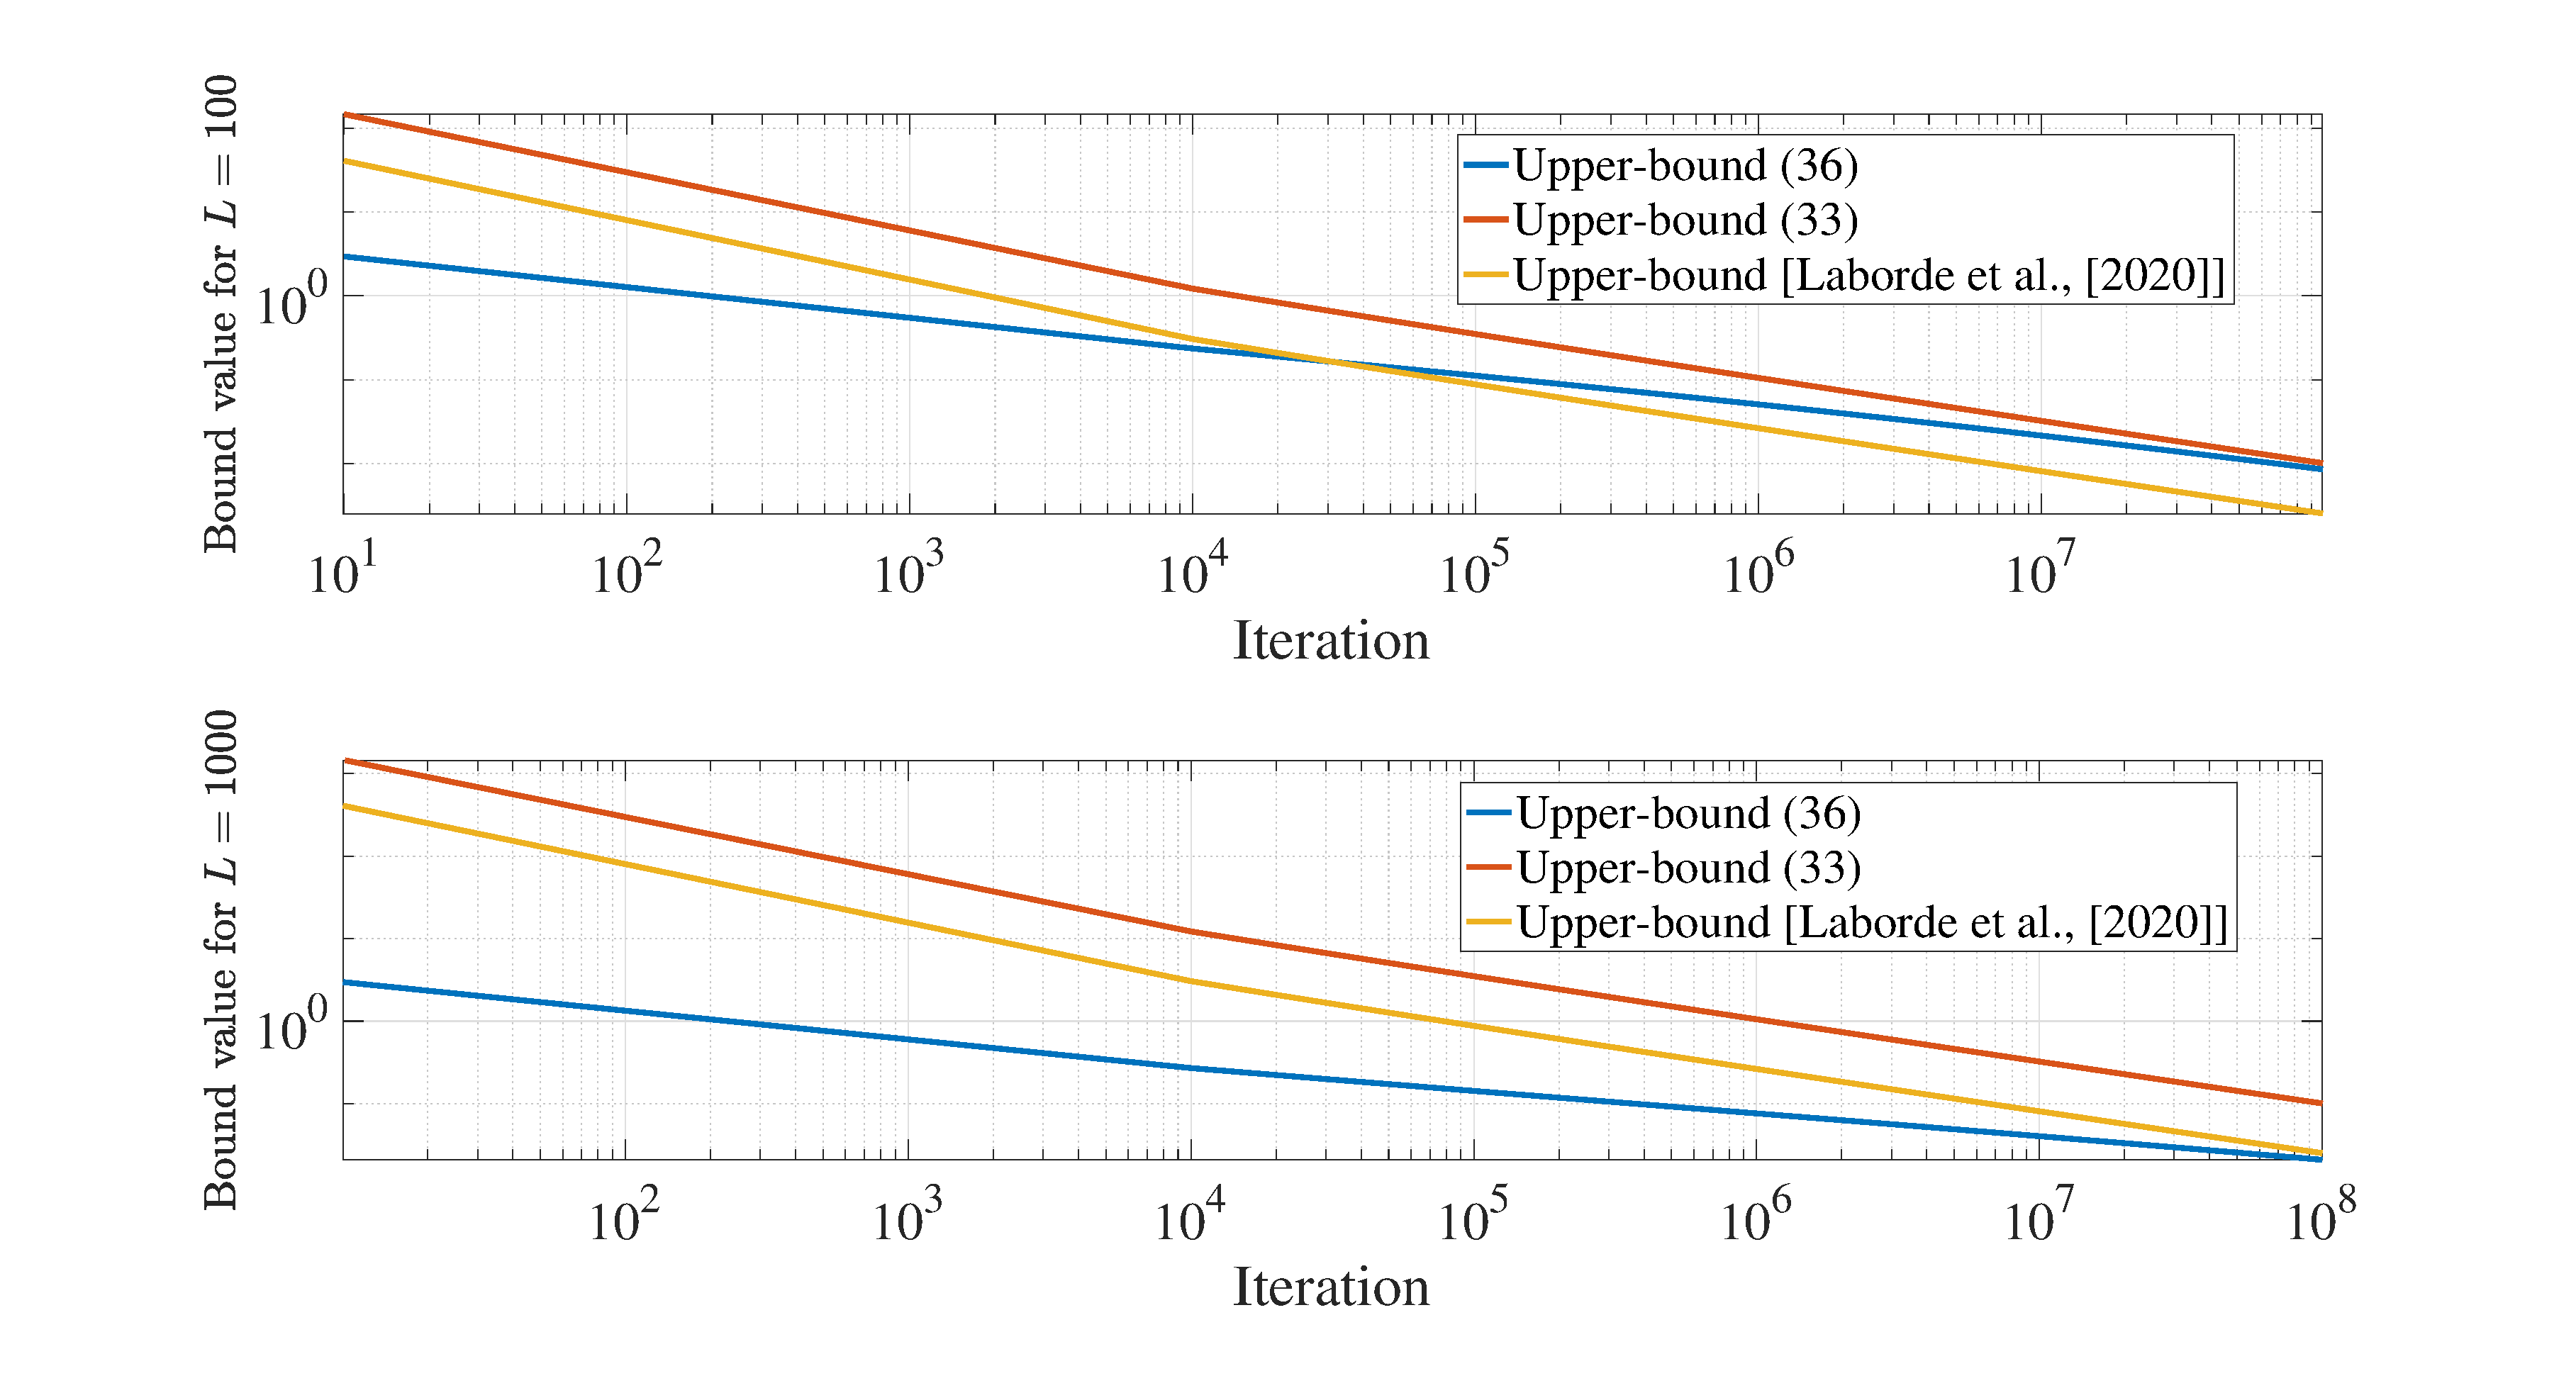
\includegraphics[width=0.45\textwidth]{NIPS 2023/Data/upperbounds.eps}\label{fig1}\subcaption{(b)}}
%\subfigure{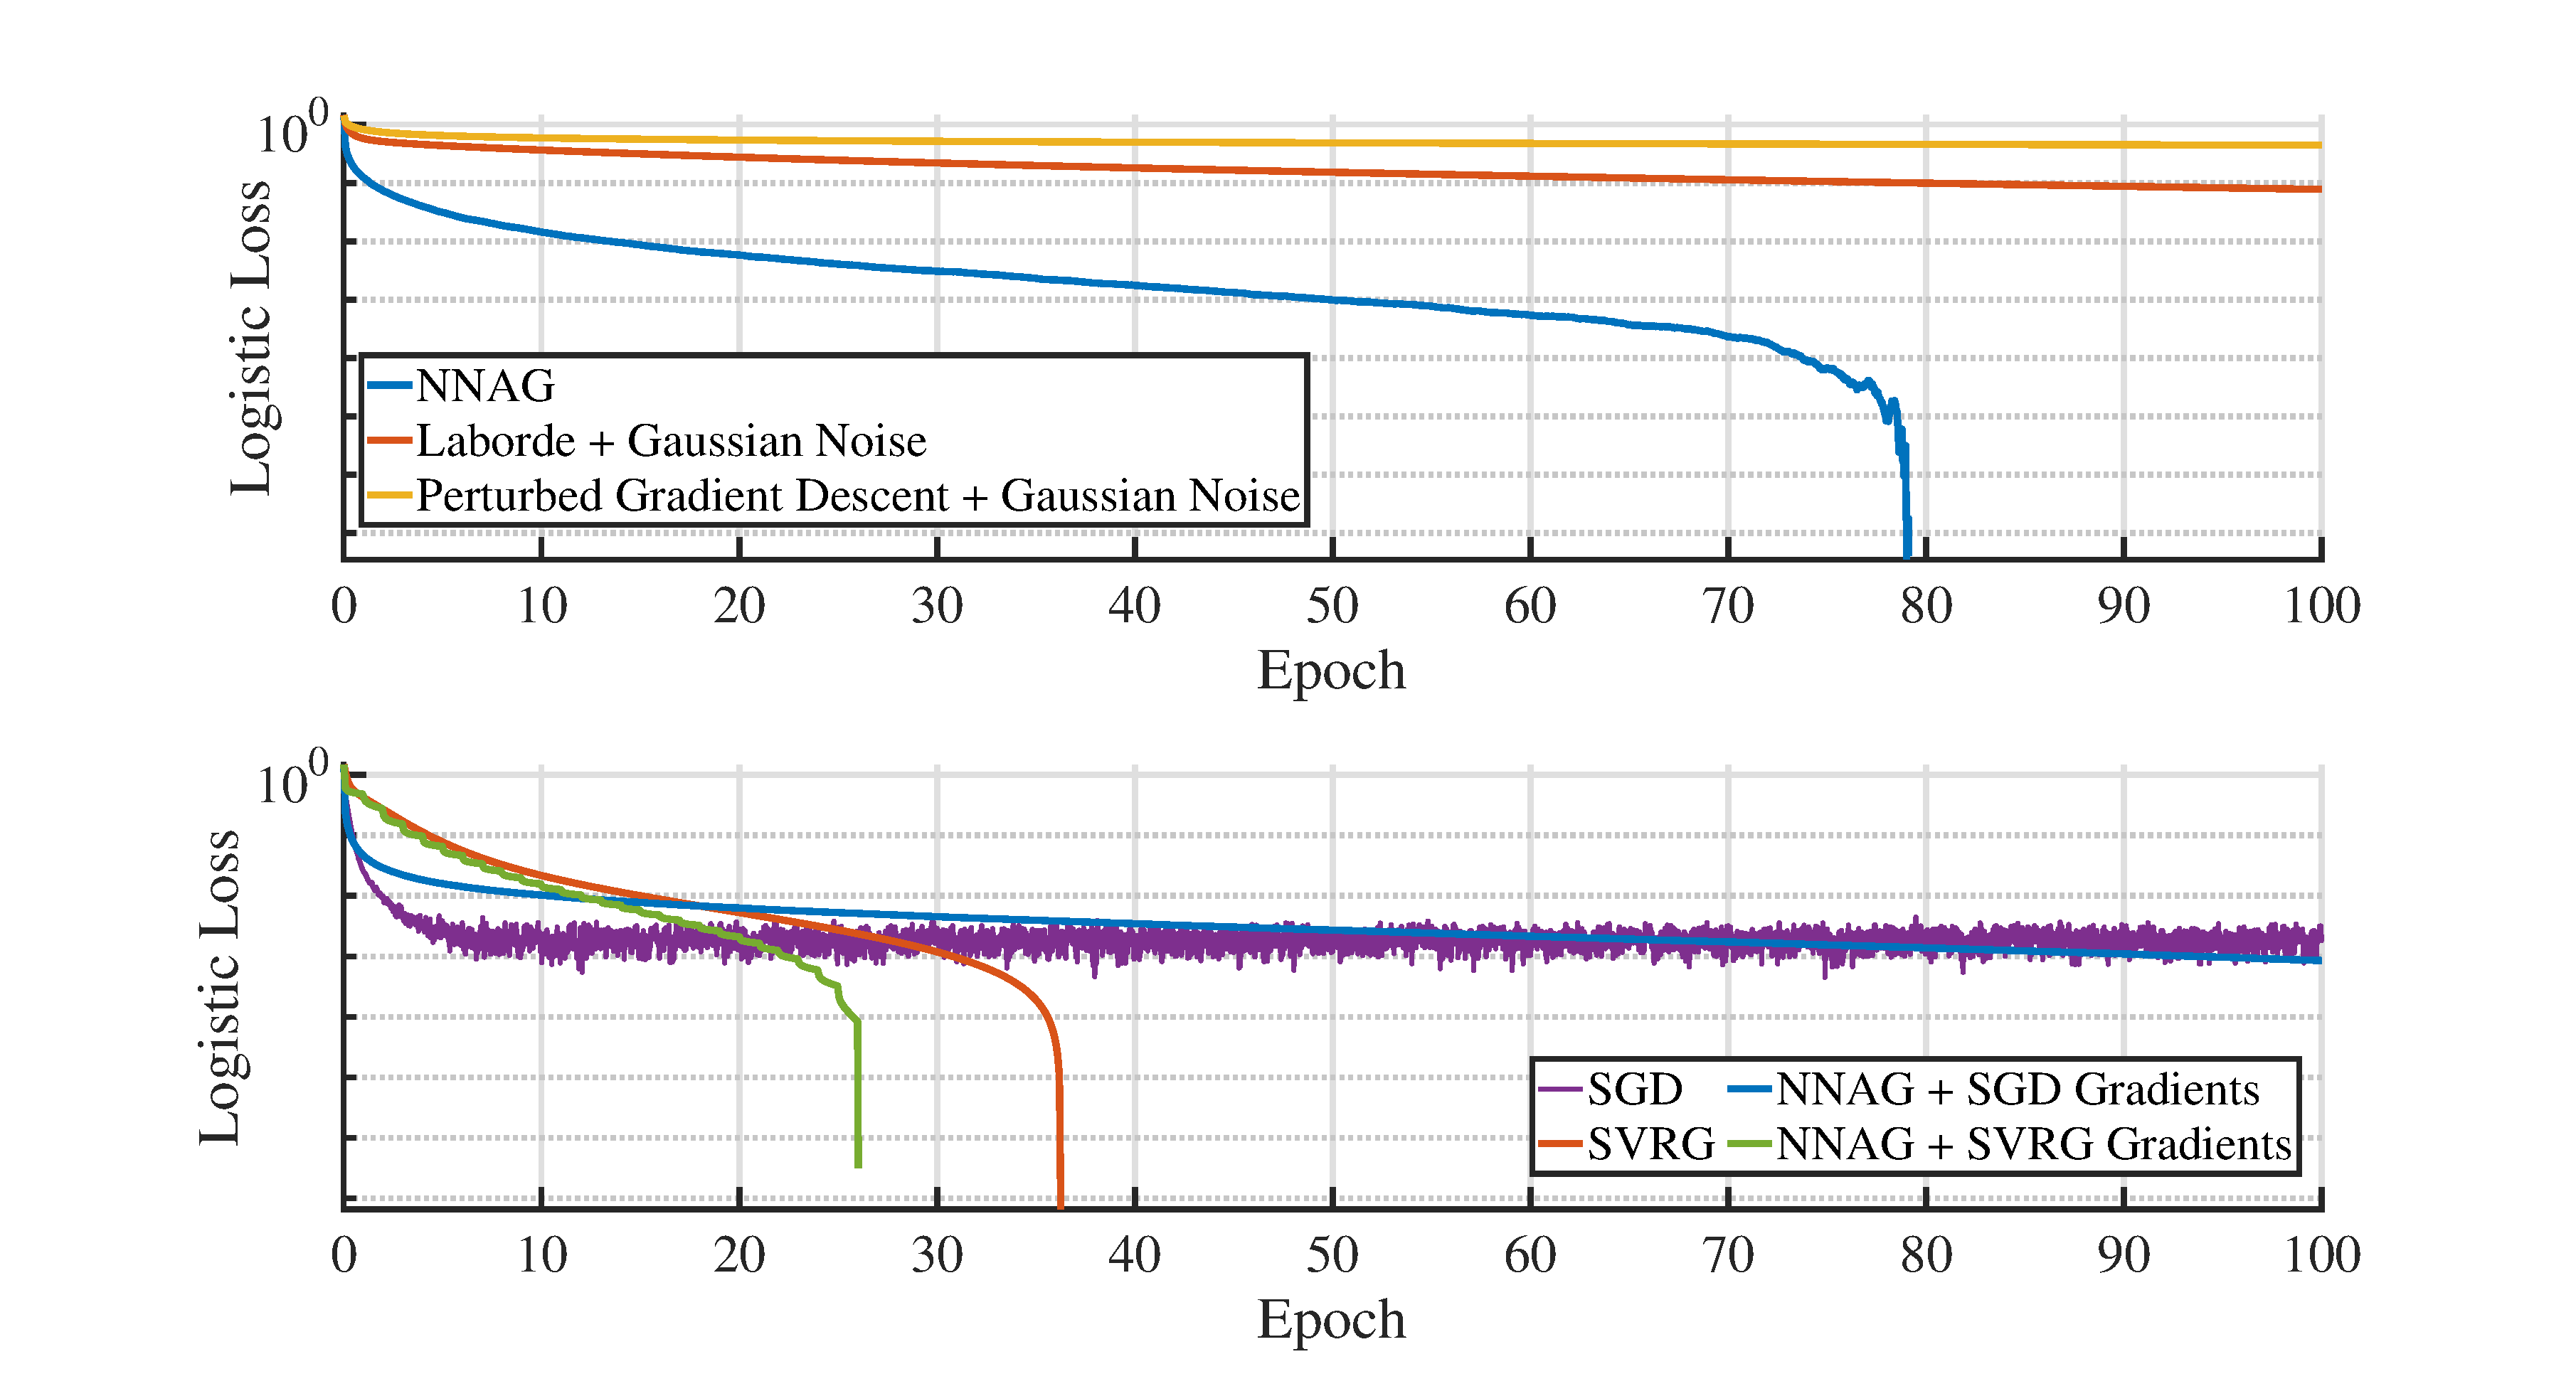
\includegraphics[width=0.45\textwidth]{NIPS 2023/Data/binary_me_sgd_svrg_corrected_me_sgd_2e5_gaussian_noise_and_no_noise_100_epochs.eps}\label{fig2}\subcaption{(a)}}
 %           \caption{(a) \(f(x)=4(L-\mu)\log(1+e^{-x})+\frac{\mu}{2}x^2\), \(L=10,\mu=10^{-3}\) and (b) 10-dimensional regularized binary classification problem with logistic loss for random data and labels of length 1000. The regularization parameter was \(\mu = 10^{-3}\).}
 %       \label{fig2_new}
%\end{figure}

\begin{figure}
  \begin{subfigure}{0.51\textwidth}
    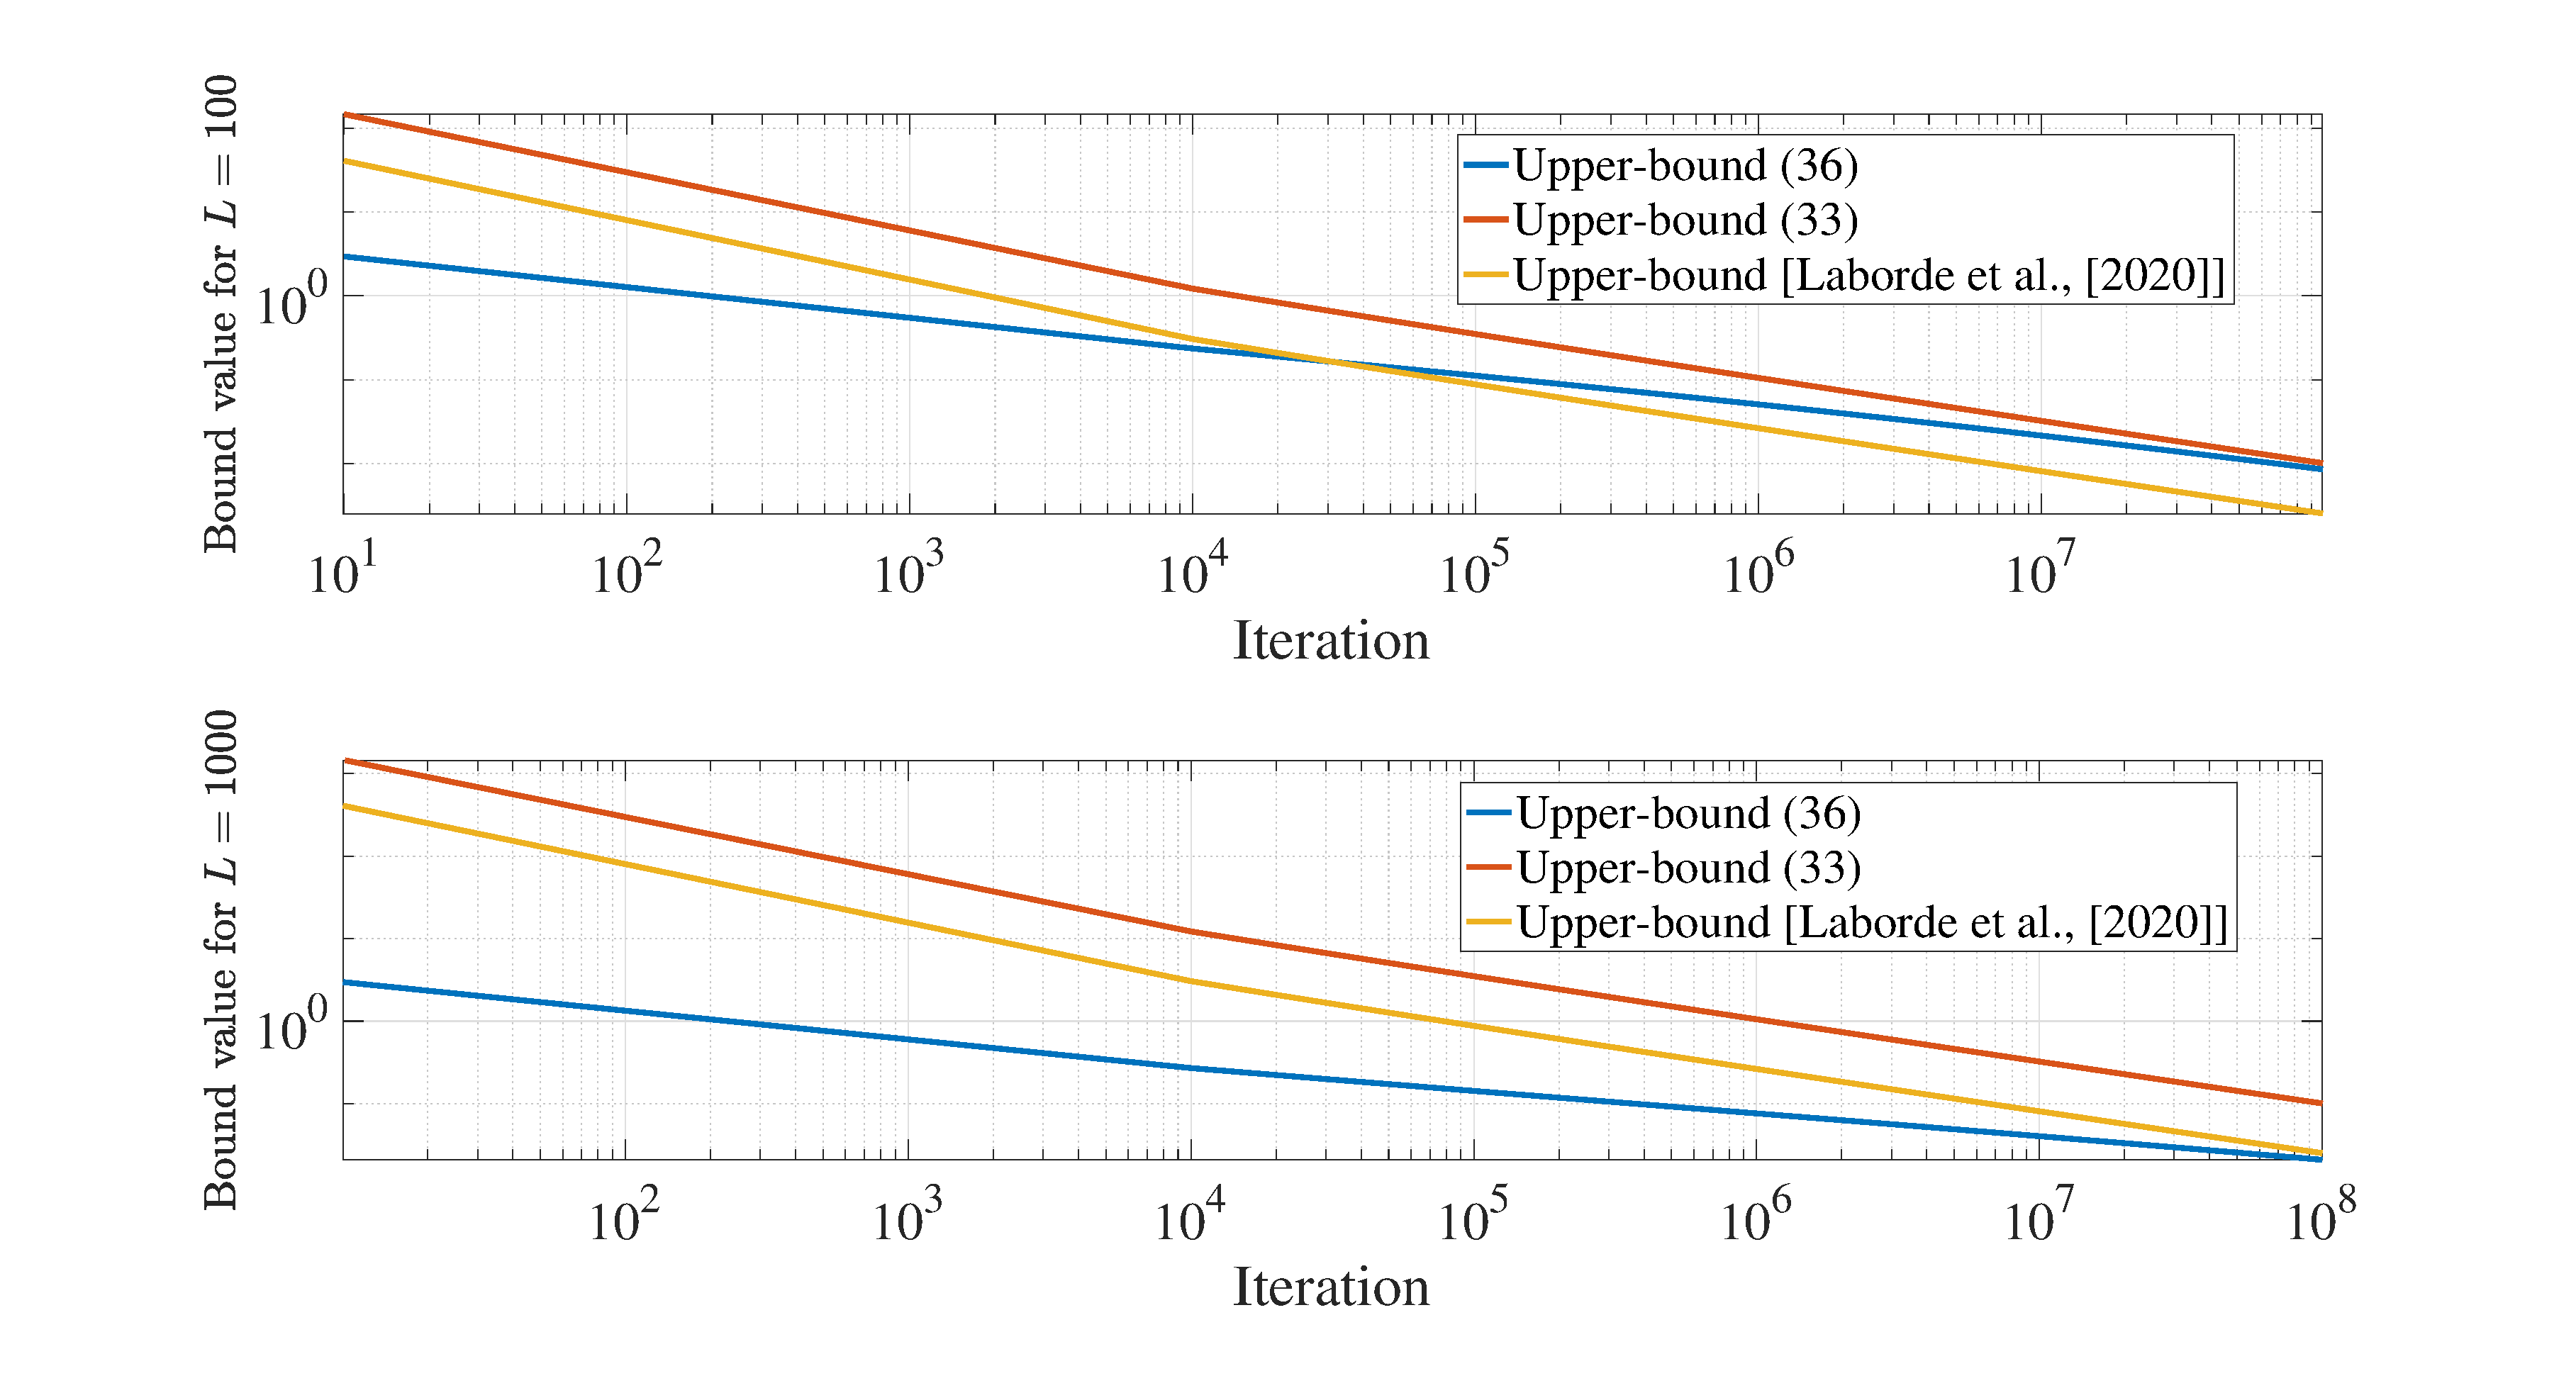
\includegraphics[width=\linewidth]{NIPS 2023/Data/upperbounds.eps}
    \caption{} \label{fig1}
  \end{subfigure}%
  \hspace*{\fill}   % maximize separation between the subfigures
  \begin{subfigure}{0.51\textwidth}
    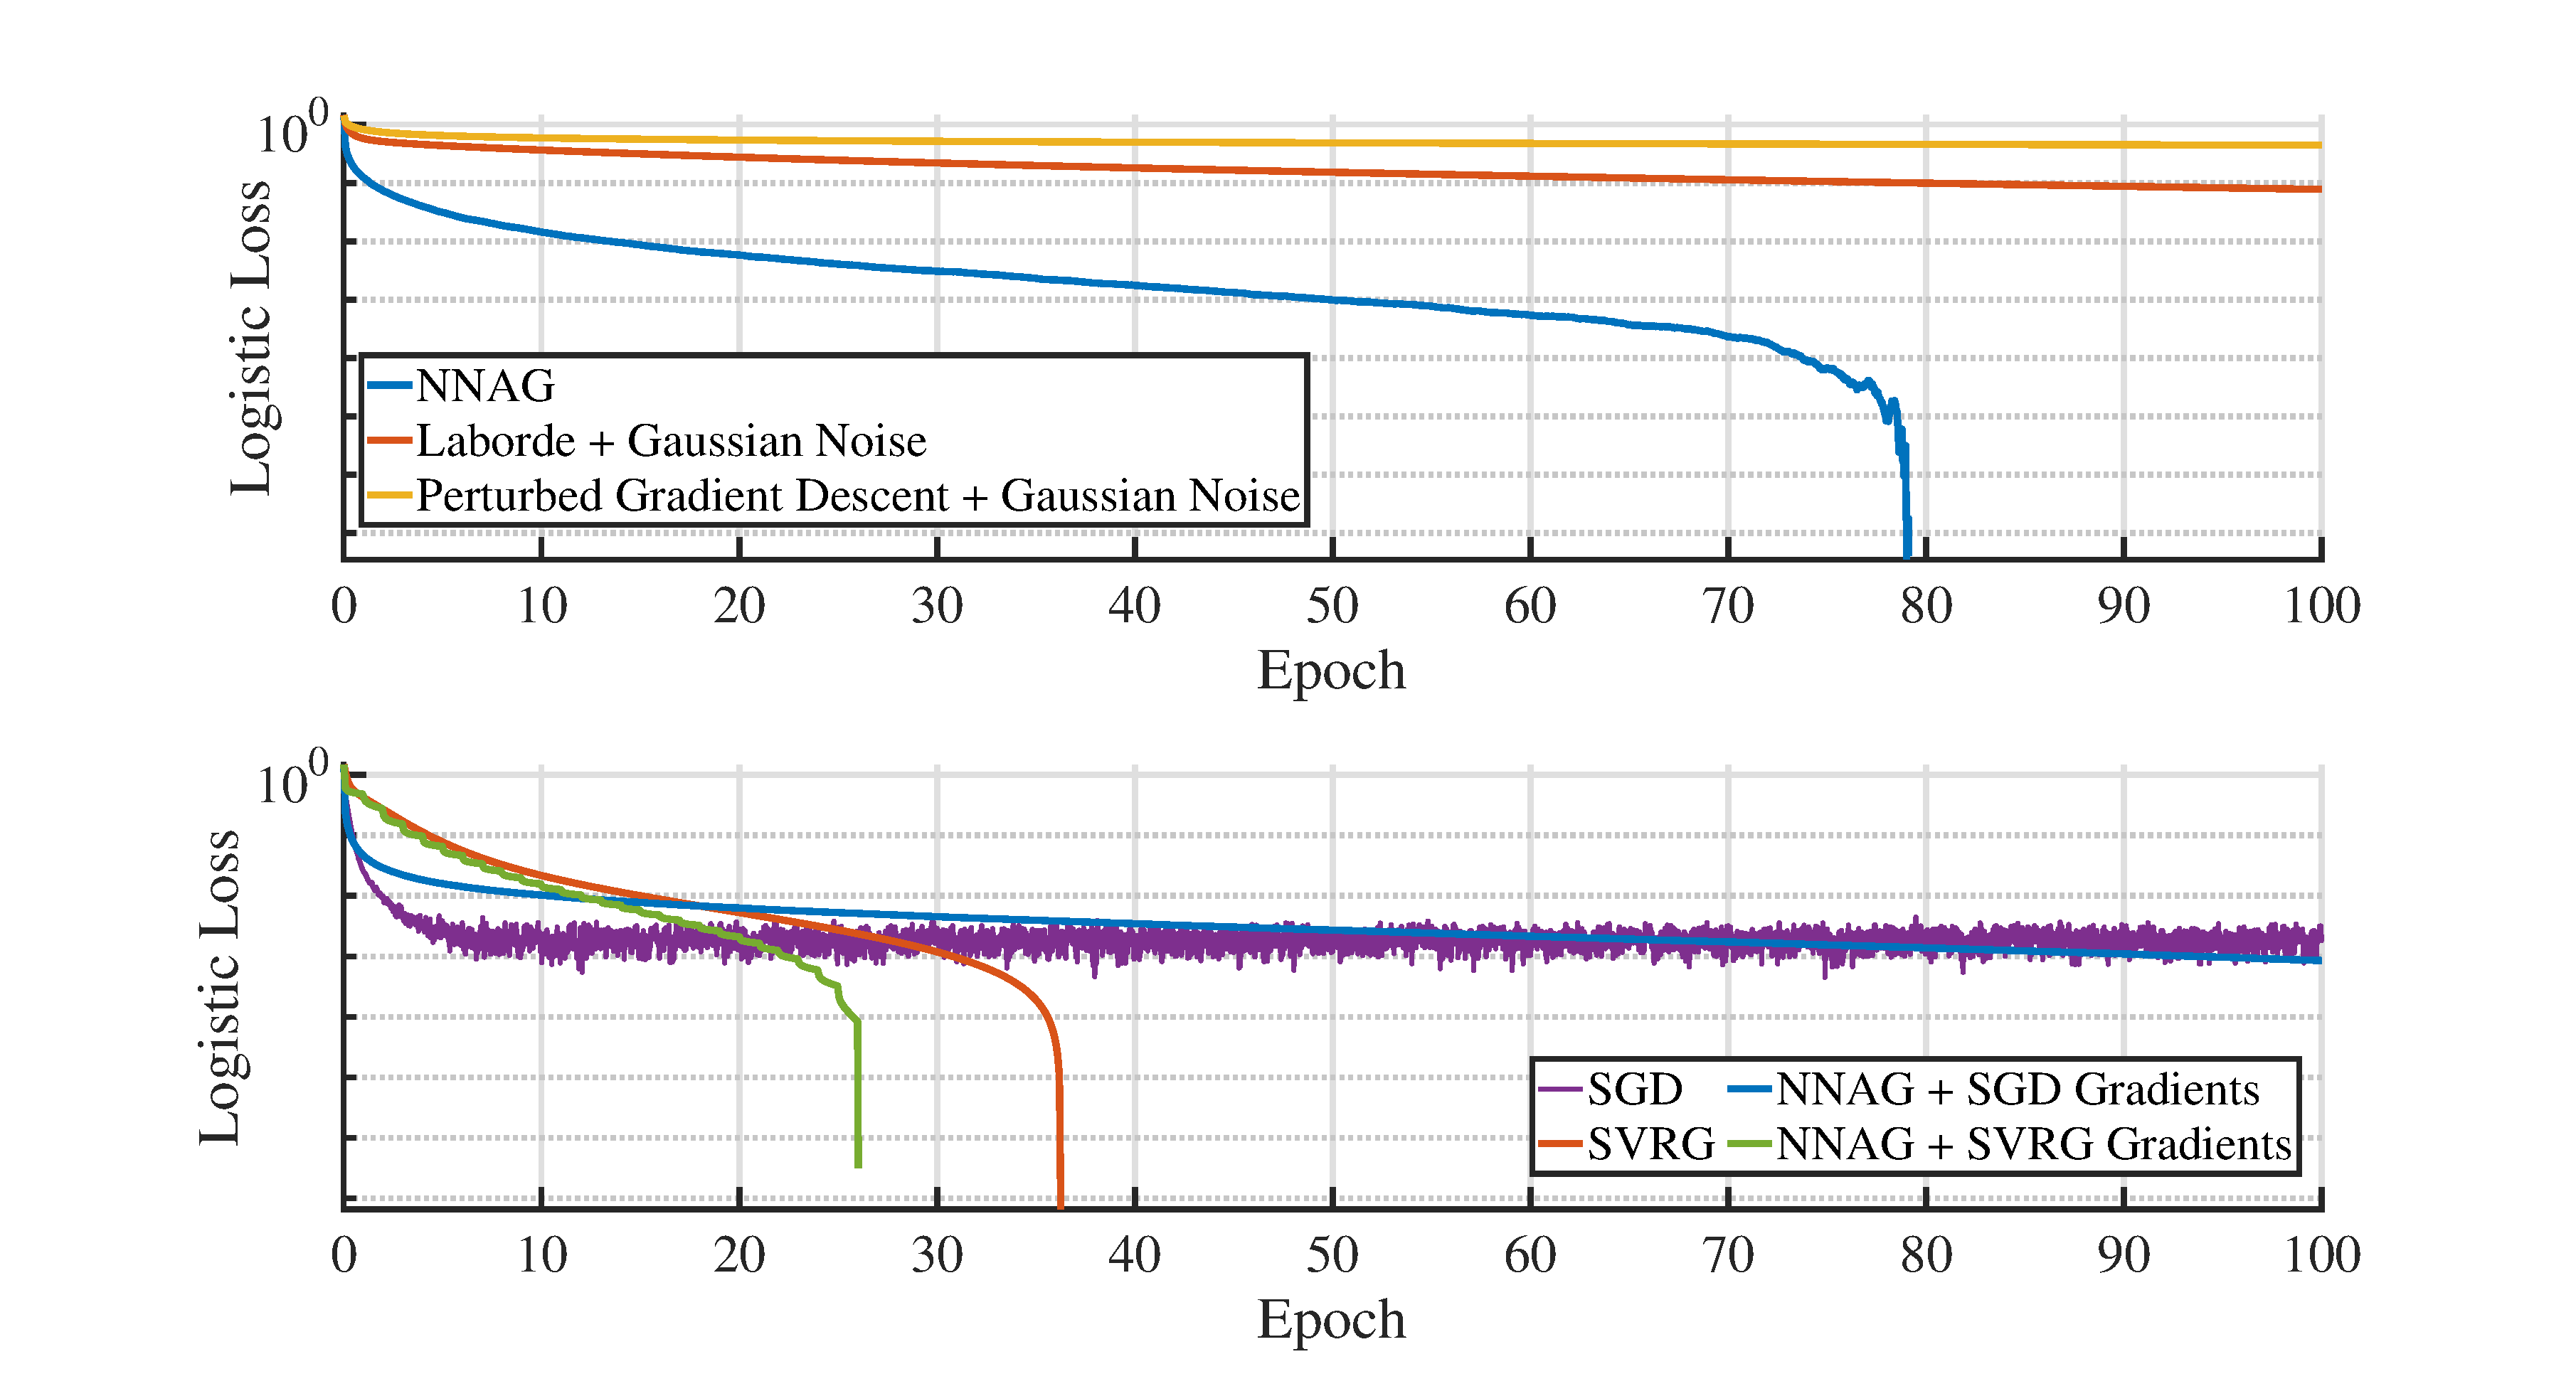
\includegraphics[width=\linewidth]{NIPS 2023/Data/binary_me_sgd_svrg_corrected_me_sgd_2e5_gaussian_noise_and_no_noise_100_epochs.eps}
    \caption{} \label{fig2}
  \end{subfigure}%
\caption{(a) Comparison of the upperbounds in this work with state of the art, (b) performance of various methods discussed in this work in binary classification problem.} \label{fig:1}
\end{figure}
\paragraph{Upperbounds}
First, we compare the bounds (\ref{Theorem7_rate2}), (\ref{conv_rate1_them6}), and Proposition 4.5 in \citep{pmlr-v108-laborde20a}. Figure \ref{fig1} depicts the result. In practical scenarios where \(L\) is large \citep{shi2022efficiently} the bound (\ref{Theorem7_rate2}) remains lower than the other two for large enough iterations. This observation has encouraged us to analyse the behaviour of NNAG in practical scenarios e.g. binary classification and CNN training tasks.
\paragraph{Binary Classification}
For this task we considered \(d=1000\) randomly generated samples of dimension \(n=10\) and labels. Then, the problem is \(\min_x \tfrac{1}{d}\sum_{i=1}^d \log(1+e^{-y_i\langle x_i,x \rangle})\) where \(y_i\) and \(x_i\) denote the \(i\)th label and sample. For comparison, we considered the perturbed gradient descent method with Gaussian noise and decreasing step-size \(s_k=1/(\sqrt{L}k^{2/3})\) (Proposition 3.4 in \citep{pmlr-v108-laborde20a}) together with accelerated noisy gradient descent (Per-FE-C) in \citep{pmlr-v108-laborde20a}. All the perturbation was done using i.i.d Gaussian noise with variance equal to one. The result is in Figure \ref{fig2} top. As shown, NNAG outperforms all the other methods in this case. In a related experiment, we mixed NNAG with SGD and SVRG. For the SGD-mixing we replaced the noisy gradients with SGD-like gradients and for the SVRG-mixing we evaluated all the gradients at the beginning of each epoch (like taking a snapshot in SVRG) and set \(t_k=0\). The result is shown in Figure 2 bottom. When mixed with SGD or SVRG, the NNAG performs better than the original methods. This stems from the generality of NNAG in terms of gradient noise and shows the potential of NNAG to mix with different methods and accelerate them.
%\begin{figure}[!ht]
%    \centering
%    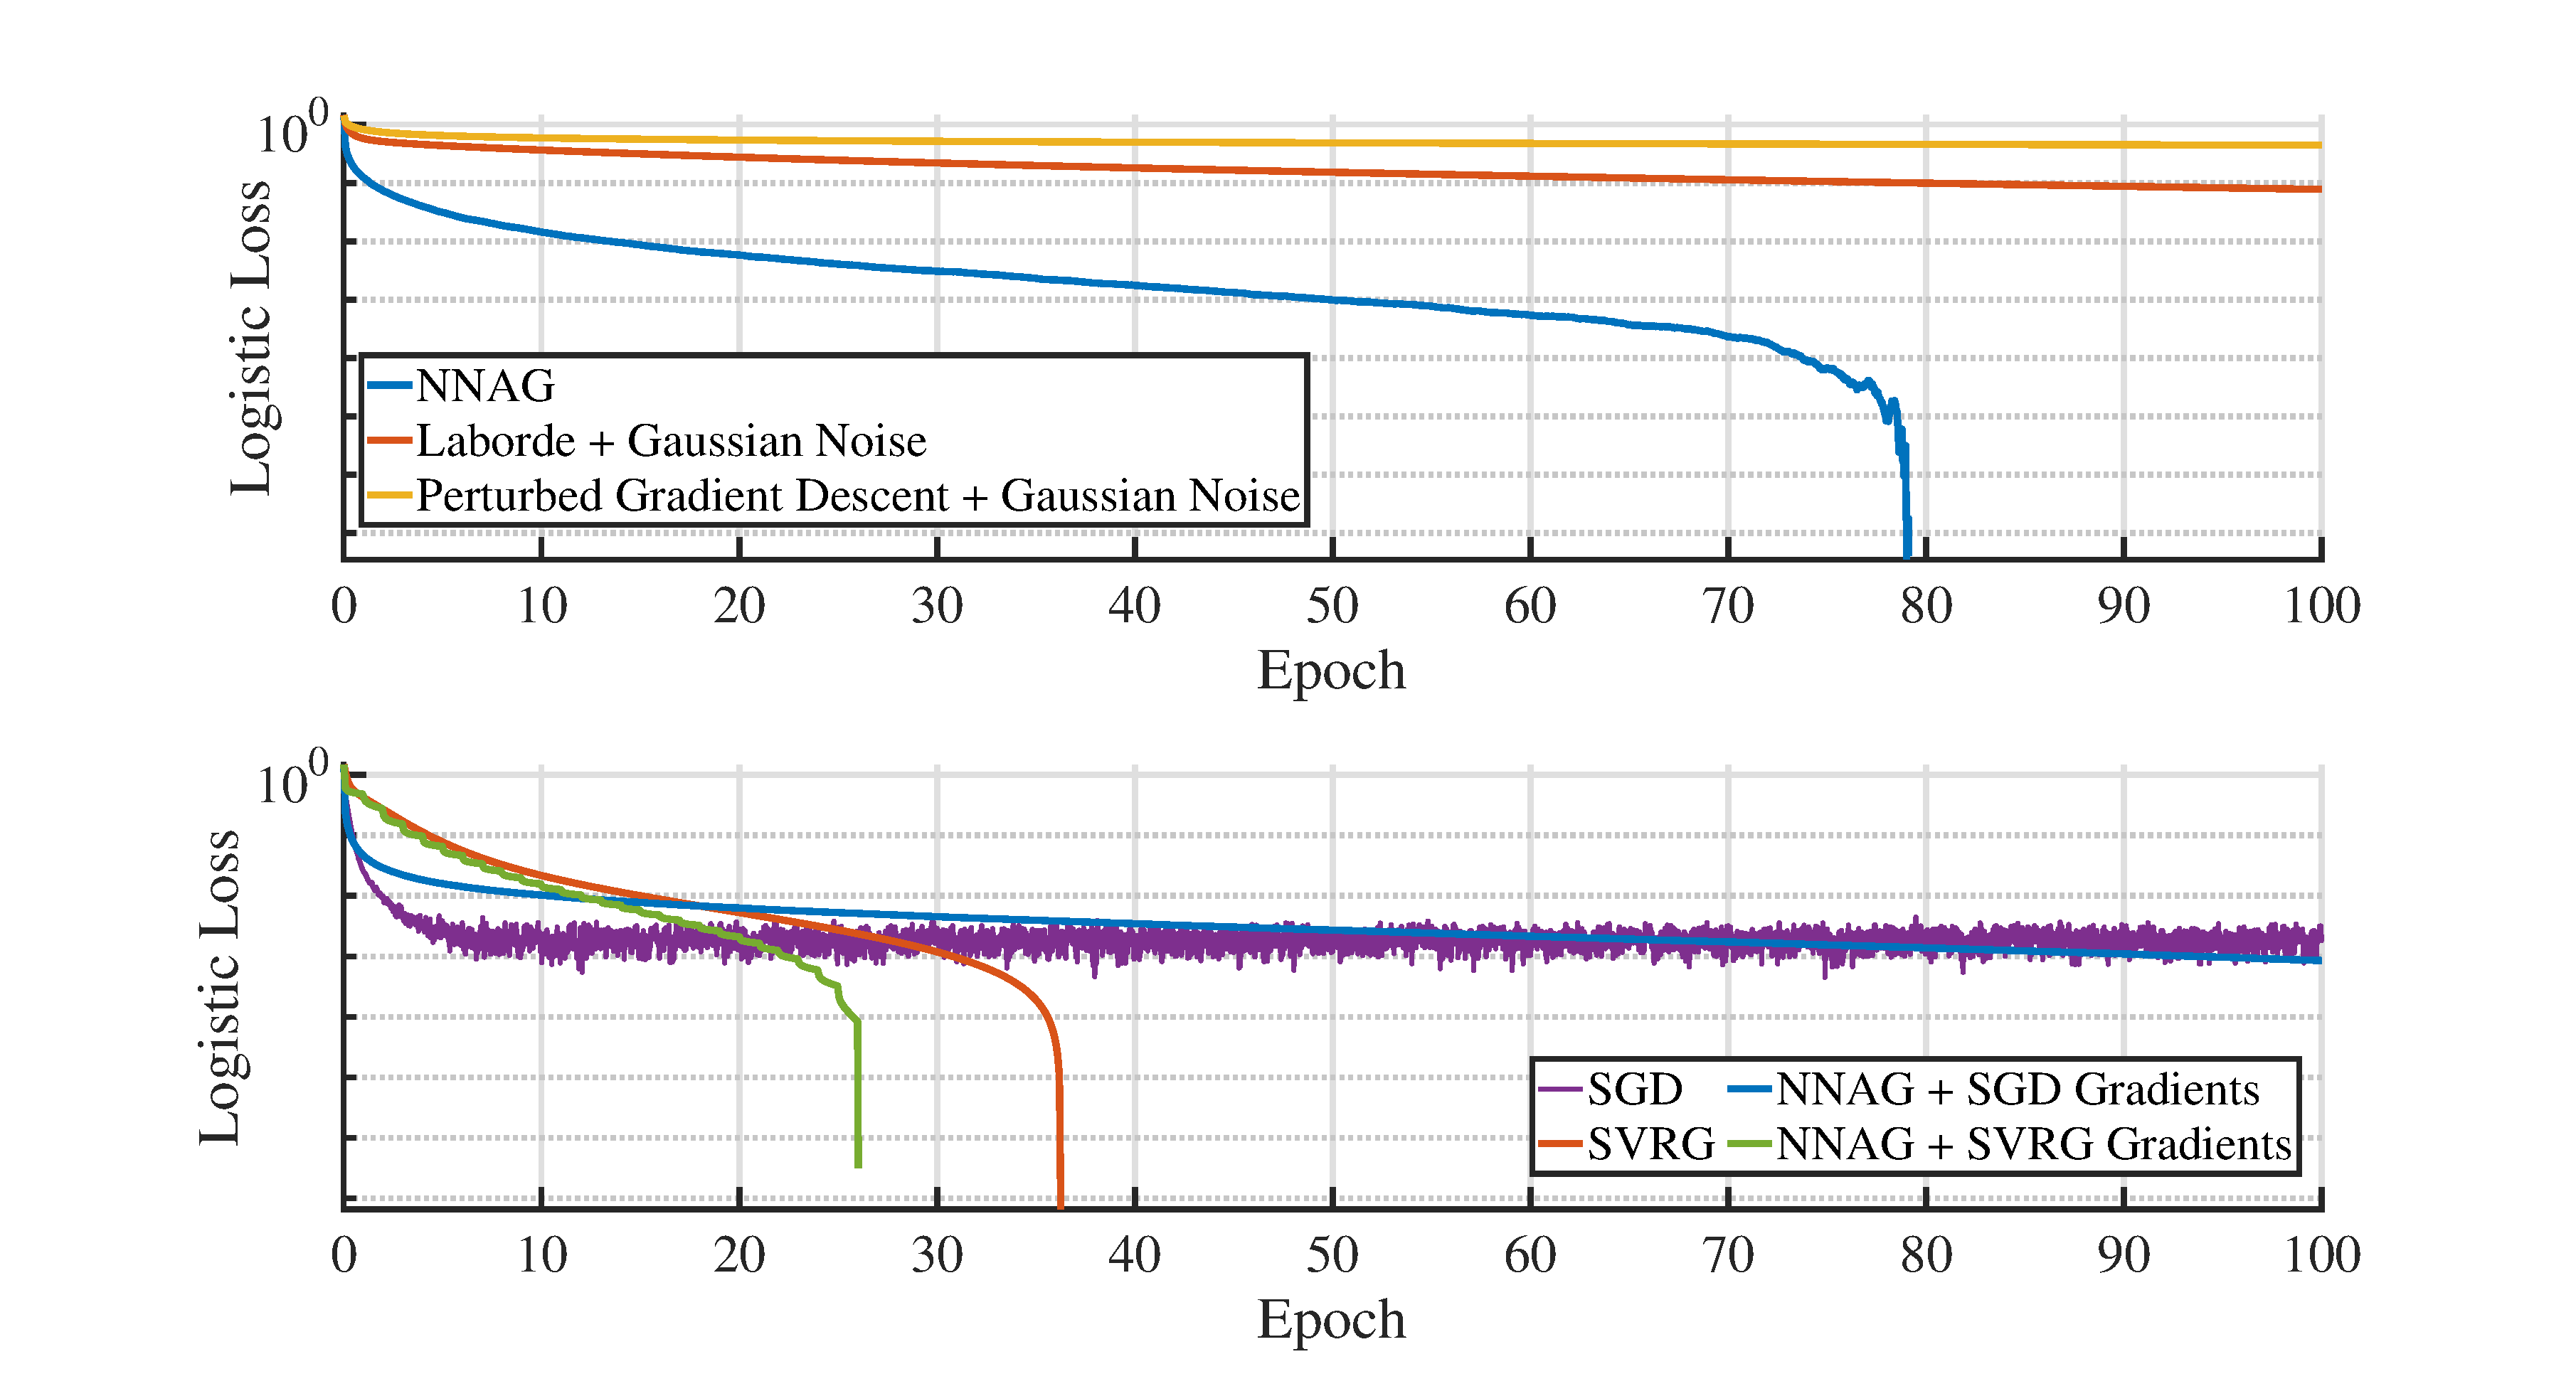
\includegraphics[width = \textwidth]{NIPS 2023/Data/binary_me_sgd_svrg_corrected_me_sgd_2e5_gaussian_noise_and_no_noise_100_epochs.eps}
%    \caption{Caption}
%    \label{fig2}
%\end{figure}
%\begin{algorithm}  
%  \caption{Counting mismatches between two packed strings  
%    \label{alg:packed-dna-hamming}}  
%  \begin{algorithmic}[5]  
%    \Require{$x$ and $y$ are packed  strings of equal length $n$}  
%    \Statex  
%    \Function{Distance}{$x, y$}  
%      \Comment{$\oplus$: bitwise exclusive-or} 
%      \For{$i \gets 1 \textrm{ to } n$}  
%        \If{$z_i \neq 0$}    
%        \EndIf  
%      \EndFor  
%      \State \Return{$\delta$}  
%    \EndFunction  
%  \end{algorithmic}  
%\end{algorithm}
\paragraph{Classification on CIFAR10}
Here we consider the non-convex task of training a CNN on CIFAR10 dataset\footnote{https://www.cs.toronto.edu/~kriz/cifar.html} through SGD, SVRG, and NNAG methods. The network consisted of two convolutional layers each followed by max pooling and 3 fully connected linear layers each followed by ReLU activation function. The results are depicted in Figure \ref{fig3}. As the figure depicts, NNAG performs comparable to SVRG and SGD methods in terms of minimizing the training error. Interestingly, the validation accuracy of NNAG is slightly better than SGD and SVRG which suggests the convergence of NNAG to a better local minima. 


\begin{figure}[!ht]
    \centering
    \begin{tikzpicture}
\begin{axis}[ name=plot_train_error,
xmin = 0 , xmax = 100,
ymin = 0 , ymax = 3,
width = 0.5*\textwidth, height = 0.4*\textwidth,
xlabel = {Epoch} , ylabel= {Training Error} ,  label style={font=\Large}, line width = 1.5
]
\addplot[red] table[x=Epoch ,y=SGD]{./NIPS 2023/Data/data_all.txt};\label{SGD_train_plot}
\addplot[orange] table[x=Epoch ,y=SVRG]{./NIPS 2023/Data/data_all.txt};\label{SVRG_train_plot}
\addplot[blue] table[x=Epoch ,y=NNAG]{./NIPS 2023/Data/data_all.txt};\label{NNAG_train_plot}
\draw[ystep=1.33cm, xstep = 1.08cm,gray,very thin] (0,0) grid (100,3);
\end{axis}

\node[anchor=north east, draw = black , fill=white]  (legend) at (plot_train_error.north east) {\begin{tabular}{l l}
    SGD & \ref{SGD_train_plot}  \\
    SVRG & \ref{SVRG_train_plot} \\
    NNAG & \ref{NNAG_train_plot}
\end{tabular}};




\begin{axis}[ name=plot_val_acc, at=(plot_train_error.outer south east),anchor = outer south west,
xmin = 0 , xmax = 100,
ymin = 0 , ymax = 0.7,
width = 0.5*\textwidth, height = 0.4*\textwidth,
xlabel = {Epoch} , ylabel= {Validation Accuracy} ,  label style={font=\Large}, line width = 1.5
]
\addplot[red] table[x=Epoch ,y=SGD]{./NIPS 2023/Data/val_acc.txt};\label{SGD_val_plot}
\addplot[orange] table[x=Epoch ,y=SVRG]{./NIPS 2023/Data/val_acc.txt};\label{SVRG_val_plot}
\addplot[blue] table[x=Epoch ,y=NNAG]{./NIPS 2023/Data/val_acc.txt};\label{NNAG_val_plot}
\draw[ystep=1.14cm, xstep = 1.08cm,gray,very thin] (0,0) grid (100,3);
\end{axis}

\node[anchor=south east, draw = black , fill=white]  (legend) at (plot_val_acc.south east) {\begin{tabular}{l l}
    SGD & \ref{SGD_val_plot}  \\
    SVRG & \ref{SVRG_val_plot} \\
    NNAG & \ref{NNAG_val_plot}
\end{tabular}};
\end{tikzpicture}
    \caption{Training error and validation accuracy of NNAG, SGD, and SVRG when used for training a simple CNN on CIFAR10 dataset.}
    \label{fig3}
\end{figure}

\section{Related Work}\label{sec_relwork}
Polyak's Heavy-Ball (HB) method was on of the first momentum-based methods which could accelerate relative to the gradient descent method \citep{Polyak1963GradientMF}. The HB method can converge globally with a rate of $\mathcal{O}(1/k)$ for every smooth convex function \citep{7330562}. However, this is not the case for every smooth strongly convex function \citep{Lessard2016AnalysisAD}. Nesterov modified the HB and introduced the NAG method. This method achieved global convergence with a rate of $\mathcal{O}(1/k^2)$ for smooth convex functions \citep{Nesterov1983AMF}. Nesterov used estimate sequence technique to show the convergence of the NAG method. This technique does not provide immediate insights toward the success of the NAG algorithm in acceleration. Thus, many have tried different approaches to understand the essence of acceleration. \par
\citep{JMLR:v17:15-084} proposed a continuous-time perspective on the NAG method. They analysed the method by letting the step-size to zero. The result of their analysis was a second-order ODE. This ODE remains the same if you repeat the analysis for the HB method. Therefore, the continuous-time analysis needed more accurate formulation. \citep{Shi2021UnderstandingTA} did the same analysis with higher accuracy which resulted in high-resolution ODEs. These ODEs were different for the HB and the NAG methods \citep{shi2019acceleration}. Extensions of this work are found in \citep{chen2022gradient,chen2022accelerating}. In \citep{chen2022gradient}, the authors use the phase-space representation of the NAG method and improve the previously found gradient norm minimization convergence rate in \citep{Shi2021UnderstandingTA}. After finishing this work, the authors found that the mentioned rate is almost the same as the rate found in this work. However, here the phase-space representation of the NAG method is not used. \par 
On similar line of work to continuous-time analysis, \citep{WibisonoE7351} introduced a variational perspective on accelerated methods. This led to a general (non-Euclidean) ODE which contained the ODE found by \citep{JMLR:v17:15-084} as a special case. Their work was based on the choice of a Lagrangian and its corresponding parameters. Since the choice of Lagrangian was not unique, \citep{wilson2021lyapunov} provided a variational perspective on different accelerated first-order methods using a second Lagrangian. \citep{7963773} found a family of accelerated dual algorithms for constrained convex minimization problem through similar variational approach. Recently, \citep{zhang2021rethinking} showed that the second-variation also plays an important role in optimality of the ODE found by \citep{JMLR:v17:15-084}. Specifically, they showed that if the time duration is long enough, then the mentioned ODE for the NAG algorithm is the saddle point to the action functional. \par
The dynamical system perspective on the NAG method was studied in \citep{muehlebach2019dynamical}. They showed that the NAG method is recovered from SIE discretization of an ODE. The mentioned ODE was not the result of a vanishing step-size argument. They found that a curvature-dependent damping term accounts for the acceleration phenomenon. Interestingly, \citep{chen2022gradient} also used similar ODE without the SIE discretization. They showed that implicit-velocity is the reason of the acceleration. In a recent analysis, \citep{muehlebach2023accelerated} explores the connections between non-smooth dynamical systems and first-order methods for constrained optimization.

\section{Conclusion}\label{sec_conclusion}
In this work, we considered unconstrained smooth convex minimization problem in the Euclidean space. Through a variational analysis on HR-ODEs, better convergence rate for the gradient norm minimization of the NAG method was achieved. In addition, we showed that the rate-matching method implicitly perturbs the LR-ODEs. Our analysis was then extended to stochastic scenarios. In particular, we proposed a method with both constant and varying step-sizes which performed comparable and sometimes better than state of the art.\par
Nesterov's oracle complexity lower bound on gradient norm minimization is \(\mathcal O({k^{-4}})\). It remains an open question to see if the NAG method can achieve this rate of convergence for gradient norm minimization. In this work we noticed that HR-ODEs follow the same external force structure. 
Triple Momentum (TM) method is the fastest known globally convergenct method for smooth strongly convex functions. However, the HR-ODE associated with the TM method cannot achieve the similar convergence rate as the TM method. One could use the external force structure proposed here to find a better HR-ODE for the TM algorithm. 
In this work, we blended our noisy stochastic scheme with other known stochastic methods (e.g. SGD and SVRG). This technique could accelerate those methods. As a future work, one can apply the same technique to other practical methods like ADAM, RMSprop, etc, and study the behaviour of the final algorithm.





\bibliographystyle{abbrvnat}
\bibliography{references}

%%%%%%%%%%%%%%%%%%%%%%%%%%%%%%%%%%%%%%%%%%%%%%%%%%%%%%%%%%%%




appendix
\section{Appendix}
\subsection{Proof of Theorem \ref{Theorem_ODE_laborde}}\label{thm1_proof}
Consider the Lyapunov function 
\begin{align}\label{lyap_theorem_C}
    \varepsilon(t)=\frac{1}{2}\|X_t+e^{-\alpha_t}\dot X_t-x^*+\sqrt{s}e^{-\alpha_t}\nabla f(X_t)\|^2+e^{\beta_t}(f(X_t)-f(x^*)).
\end{align}
Taking derivative with respect to $t$ gives
\begin{align}\label{prf_thm1_eqn1}
    \frac{d \varepsilon}{dt}=&\langle \frac{d}{dt}(X_t+e^{-\alpha_t}\dot X_t-x^*+\sqrt{s}e^{-\alpha_t}\nabla f(X_t)),X_t+e^{-\alpha_t}\dot X_t-x^*+\sqrt{s}e^{-\alpha_t}\nabla f(X_t)\rangle\nonumber\\
    & +\dot \beta_t e^{\beta_t}(f(X_t)-f(x^*))+e^{\beta_t}\langle \nabla f(X_t), \dot X_t\rangle.
\end{align}
Note that (\ref{HR_general_ODE_F_laborde}) can be represented as
\begin{align}\label{HR_general_der_format_laborde}
    \frac{d}{dt}\left[X_t+e^{-\alpha_t}\dot X_t+\sqrt{s}e^{-\alpha_t}\nabla f(X_t)\right]=-e^{\alpha_t+\beta_t}\nabla f(X_t).
\end{align}
Using (\ref{HR_general_der_format_laborde}) in (\ref{prf_thm1_eqn1}) we have
\begin{align}
     \frac{d \varepsilon}{dt}=& \langle -e^{\alpha_t+\beta_t}\nabla f(X_t),X_t+e^{-\alpha_t}\dot X_t-x^*+\sqrt{s}e^{-\alpha_t}\nabla f(X_t) \rangle \nonumber \\
     &+\dot \beta_t e^{\beta_t}(f(X_t)-f(x^*))+e^{\beta_t}\dot X_t\nabla f(X_t)\nonumber\\
     &= -e^{\alpha_t+\beta_t}\langle\nabla f(X_t),X_t-x^*\rangle -e^{\beta_t}\langle \nabla f(X_t),\dot X_t\rangle -\sqrt{s}e^{\beta_t}\|\nabla f(X_t)\|^2\nonumber\\
     &+\dot \beta_te^{\beta_t}(f(X_t)-f(x^*))+e^{\beta_t}\langle \nabla f(X_t),\dot X_t \rangle\nonumber\\
     & \overset{\text{(\ref{convexity}})}{\leq} -e^{\alpha_t+\beta_t}(f(X_t)-f(x^*))+\dot \beta_te^{\beta_t}(f(X_t)-f(x^*))\nonumber\\
     & = -e^{\beta_t}\left[(e^{\alpha_t}-\dot \beta_t)(f(X_t)-f(x^*))\right].\nonumber
\end{align}
Utilizing the ideal scaling condition $\dot \beta_t\leq e^{\alpha_t}$ we have
\begin{align}
     \frac{d \varepsilon}{dt}\leq 0.\nonumber
\end{align}
Thus, for the initialization point $t_0$ we have
$$e^{\beta_t}(f(X_t)-f(x^*))\leq \varepsilon(t)\leq \varepsilon(t_0),$$
and the proof is complete.
\subsection{Proof of Theorem \ref{Theorem_ODE_Shi}}\label{thm3_proof}
Consider the Lyapunov function 
\begin{align}\label{lyap_theorem3}
    \varepsilon(t)=\frac{1}{2}\|X_t+e^{-\alpha_t}\dot X_t-x^*+\sqrt{s}e^{-\alpha_t}\nabla f(X_t)\|^2+(e^{\beta_t}+\sqrt{s}e^{-2\alpha_t}\dot \beta_t)(f(X_t)-f(x^*)).
\end{align}
Taking derivative with respect to $t$ gives
\begin{align}\label{prf_thm3_eqn1}
    \frac{d \varepsilon}{dt}=&\langle \frac{d}{dt}(X_t+e^{-\alpha_t}\dot X_t-x^*+\sqrt{s}e^{-\alpha_t}\nabla f(X_t)),X_t+e^{-\alpha_t}\dot X_t-x^*+\sqrt{s}e^{-\alpha_t}\nabla f(X_t)\rangle\nonumber\\
    & +(\dot \beta_te^{\beta_t}-\sqrt{s}(2\dot \alpha_t)e^{-2\alpha_t}\dot \beta_t +\sqrt{s}e^{-\alpha_t}\Ddot{\beta_t})(f(X_t)-f(x^*))\nonumber\\
    &+(e^{\beta_t}+\sqrt{s}e^{-2\alpha_t}\dot \beta_t)\dot X_t\nabla f(X_t).
\end{align}
Note that (\ref{HR_general_ODE_F_laborde}) can be represented as
\begin{align}\label{HR_general_der_format_Shi}
    \frac{d}{dt}\left[X_t+e^{-\alpha_t}\dot X_t+\sqrt{s}e^{-\alpha_t}\nabla f(X_t)\right]=-\left(e^{\alpha_t+\beta_t}+\sqrt{s}e^{-\alpha_t}\dot \beta_t \right)\nabla f(X_t).
\end{align}
Using (\ref{HR_general_der_format_Shi}) in (\ref{prf_thm3_eqn1}) we have
\begin{align}
     \frac{d \varepsilon}{dt}=& \langle -\left(e^{\alpha_t+\beta_t}+\sqrt{s}e^{-\alpha_t}\dot \beta_t \right)\nabla f(X_t),X_t+e^{-\alpha_t}\dot X_t-x^*+\sqrt{s}e^{-\alpha_t}\nabla f(X_t) \rangle \nonumber \\
     &+(\dot \beta_te^{\beta_t}-\sqrt{s}(2\dot \alpha_t)e^{-2\alpha_t}\dot \beta_t +\sqrt{s}e^{-2\alpha_t}\Ddot{\beta_t})(f(X_t)-f(x^*))\nonumber\\
    &+(e^{\beta_t}+\sqrt{s}e^{-2\alpha_t}\dot \beta_t)\langle\nabla f(X_t),\dot X_t\rangle,\nonumber\\
     &= -\left(e^{\alpha_t+\beta_t}+\sqrt{s}e^{-\alpha_t}\dot \beta_t \right)\langle\nabla f(X_t),X_t-x^*\rangle -\left(e^{\beta_t}+\sqrt{s}e^{-2\alpha_t}\dot \beta_t \right)\langle \nabla f(X_t),\dot X_t\rangle \nonumber\\
     &-\sqrt{s}\left(e^{\beta_t}+\sqrt{s}e^{-2\alpha_t}\dot \beta_t \right)\|\nabla f(X_t)\|^2\nonumber\\
     &+(\dot \beta_te^{\beta_t}-\sqrt{s}(2\dot \alpha_t)e^{-2\alpha_t}\dot \beta_t +\sqrt{s}e^{-2\alpha_t}\Ddot{\beta_t})(f(X_t)-f(x^*))\nonumber\\
    &+(e^{\beta_t}+\sqrt{s}e^{-2\alpha_t}\dot \beta_t)\langle\nabla f(X_t),\dot X_t\rangle,\nonumber\\
     & \overset{\text{(\ref{convexity}})}{\leq} -\left(e^{\alpha_t+\beta_t}+\sqrt{s}e^{-\alpha_t}\dot \beta_t \right)(f(X_t)-f(x^*))\nonumber\\
     &+(\dot \beta_te^{\beta_t}-\sqrt{s}(2\dot \alpha_t)e^{-2\alpha_t}\dot \beta_t +\sqrt{s}e^{-2\alpha_t}\Ddot{\beta_t})(f(X_t)-f(x^*)),\nonumber\\
     & = -\left[e^{\beta_t}(e^{\alpha_t}-\dot \beta_t)+\sqrt{s}e^{-\alpha_t}(\dot \beta_t+2\dot \alpha_t e^{-\alpha_t}\dot \beta_t-e^{-\alpha_t}\Ddot{\beta}_t)\right](f(X_t)-f(x^*)).\nonumber
\end{align}
Utilizing the modified ideal scaling conditions $\dot \beta_t\leq e^{\alpha_t}$ and $\Ddot{\beta}_t\leq e^{\alpha_t}\dot \beta_t + 2\dot \alpha_t \dot \beta_t$ we have
\begin{align}
     \frac{d \varepsilon}{dt}\leq 0.\nonumber
\end{align}
Thus, for the initialization point $t_0$ we have
$$(e^{\beta_t}+\sqrt{s}e^{-2\alpha_t}\dot \beta_t)(f(X_t)-f(x^*))\leq \varepsilon(t)\leq \varepsilon(t_0),$$
and the proof is complete.
\subsection{Proof of Theorem \ref{Theorem3_1}}\label{thm4_proof}
Consider the Lyapunov function
    \begin{align}\label{thm32_eqn_1}
        \varepsilon(t) = e^{\beta_t}\left(\frac{\mu}{2}\|X_t-x^*+e^{-\alpha_t}\dot X_t+\frac{\sqrt{s}e^{\alpha_t}}{\mu}\nabla f(X_t)\|^2+f(X_t)-f(x^*)\right).
    \end{align}
    Taking derivative w.r.t. time gives
    \begin{align}\label{thm32_eqn_2}
       \frac{d\varepsilon(t)}{dt}&=\dot \beta e^{\beta_t}\left(\frac{\mu}{2}\|X_t-x^*+e^{-\alpha_t}\dot X_t+\frac{\sqrt{s}e^{\alpha_t}}{\mu}\nabla f(X_t)\|^2+f(X_t)-f(x^*)\right)\nonumber\\
       & + \mu e^{\beta_t}\left\langle \dot X_t-\dot \alpha_t e^{-\alpha_t}\dot X_t + e^{-\alpha_t}\Ddot{X}_t +\frac{\sqrt{s}}{\mu}\dot \alpha_te^{\alpha_t}\nabla f(X_t)+\frac{\sqrt{s}}{\mu}e^{\alpha_t}\nabla ^2f(X_t)\dot X_t\right.\nonumber\\
       &\left. ,X_t-x^*+e^{-\alpha_t}\dot X_t+\frac{\sqrt{s}e^{\alpha_t}}{\mu}\nabla f(X_t)\right\rangle+e^{\beta_t}\langle \nabla f(X_t),\dot X_t \rangle.
    \end{align}
    Next, we will use (\ref{sc_eqn1}) in (\ref{thm32_eqn_2})
    \begin{align}\label{thm32_eqn_3}
        \frac{d\varepsilon(t)}{dt}&=\dot \beta e^{\beta_t}\left(\frac{\mu}{2}\|X_t-x^*+e^{-\alpha_t}\dot X_t+\frac{\sqrt{s}e^{\alpha_t}}{\mu}\nabla f(X_t)\|^2+f(X_t)-f(x^*)\right)\nonumber\\
       & + \mu e^{\beta_t}\left\langle \dot X_t-e^{-\alpha_t}(\dot \gamma_t+\dot \beta_t)\dot X_t  +\frac{e^{\alpha_t }}{\mu}(\sqrt{s}(\dot \alpha_t-\dot \beta_t)-1)\nabla f(X_t)\right.\nonumber\\
       &\left. ,X-x^*+e^{-\alpha_t}\dot X_t+\frac{\sqrt{s}e^{\alpha_t}}{\mu}\nabla f(X_t)\right\rangle+e^{\beta_t}\langle \nabla f(X_t),\dot X_t \rangle,\nonumber\\
   &= \dot \beta_t e^{\beta_t}\left(\frac{\mu}{2}\left[\|X_t-x^*\|^2+e^{-2\alpha_t}\|\dot X_t\|^2+\|\frac{\sqrt{s}e^{\alpha_t}}{\mu}\nabla f(X_t)\|^2+2e^{-\alpha_t}\langle X_t-x^*,\dot X_t\rangle\right.\right.\nonumber\\
   &\left.\left.+\frac{2\sqrt{s}e^{\alpha_t}}{\mu}\langle X_t-x^*,\nabla f(X_t) \rangle+ \frac{2\sqrt{s}}{\mu}\langle \nabla f(X_t),\dot X_t \rangle\right]\right)+\dot \beta_t e^{\beta_t} (f(X_t)-f(x^*) )\nonumber\\
   & +\mu e^{\beta_t}\left[ (1-e^{-\alpha_t}(\dot \gamma_t+\dot \beta_t))\langle \dot X_t,X_t-x^*\rangle+ e^{-\alpha_t}(1-e^{-\alpha_t}(\dot \gamma_t+\dot \beta_t))\|\dot X_t\|^2 \right.\nonumber\\
   & +\frac{\sqrt{s}e^{\alpha_t}}{\mu}(1-e^{-\alpha_t}(\dot \gamma_t+\dot \beta_t))\langle \dot X_t,\nabla f(X_t) \rangle + \frac{e^{\alpha_t }}{\mu}(\sqrt{s}(\dot \alpha_t-\dot \beta_t)-1)\langle \nabla f(X_t) ,X_t-x^*\rangle\nonumber\\
   & \left.+ \frac{(\sqrt{s}(\dot \alpha_t-\dot \beta_t)-1)}{\mu}\langle \nabla f(X_t),\dot X_t \rangle+\frac{\sqrt{s}e^{2\alpha_t}}{\mu^2}(\sqrt{s}(\dot \alpha_t-\dot \beta_t)-1)\|\nabla f(X_t)\|^2\right]\nonumber\\
   & + e^{\beta_t}\langle \nabla f(X_t),\dot X_t \rangle.
    \end{align}
    Now, using strong convexity of $f$ and applying $ \alpha_t=\alpha$, $\dot \beta\geq 0$, $\dot \gamma_t=e^{\alpha_t}$, and $\dot \beta_t\leq e^{\alpha_t}$ gives
    \begin{align}\label{thm32_eqn_4}
        \frac{d\varepsilon(t)}{dt}&\leq-\dot \beta_t e^{\beta_t}\|\sqrt{\frac{\mu}{2}}e^{-\alpha_t}\dot X_t\|^2-\sqrt{s}e^{\beta_t}\dot \beta_t\langle \dot X_t,\nabla f(X_t) \rangle-\dot \beta_t e^{\beta_t}\|\frac{\sqrt{s}e^{\alpha_t}}{\sqrt{2\mu}}\nabla f(X_t)\|^2\nonumber\\
        &=-\dot \beta_t e^{\beta_t} \|    \sqrt{\frac{\mu}{2}}e^{-\alpha_t}\dot X_t+  \frac{\sqrt{s}e^{\alpha_t}}{\sqrt{2\mu}}\nabla f(X_t)\|^2\leq 0,
    \end{align}
    and therefore, 
    $$e^{\beta_t}(f(X_t)-f(x^*))\leq \varepsilon(t)\leq \varepsilon(0)$$
    and the proof is complete.
\subsection{Proof of Theorem \ref{theorem4}}\label{thm5_proof}
    Take the Lyapunov function 
\begin{align}\label{Lyapunov_function}
    \varepsilon(k) = \frac{s(k+2)k}{4}(f(x_k)-f(x^*))+\frac{1}{2}\|x_{k+1}-x^*+\frac{k}{2}(x_{k+1}-x_k)+\frac{ks}{2}\nabla f(x_k)\|^2.
\end{align}
The choice of Lyapunov function is the same as \citep{Shi2021UnderstandingTA}. Note that the second term is equivalent to $\frac{1}{2}\|v_k-x^*\|^2$ through the first line of the update rule (\ref{new_algorithm}). Next, we will show that 
\begin{align}\label{Lyap_1}
    \varepsilon(k+1)-\varepsilon(k)\leq -\frac{s^2k(k+2)}{8}\|\nabla f(x_k)\|^2.
\end{align}
Using (\ref{Lyapunov_function}) we have
\begin{align}\label{Lyap_2}
    \varepsilon(k+1)-\varepsilon(k)&=\frac{s(k+3)(k+1)}{4}(f(x_{k+1})-f(x^*))+\frac{1}{2}\|v_{k+1}-x^*\|^2\nonumber\\
    & - \frac{s(k+2)(k)}{4}(f(x_{k})-f(x^*))+\frac{1}{2}\|v_{k}-x^*\|^2\nonumber\\
    &=\frac{s(k+2)k}{4}(f(x_{k+1})-f(x_k))+\frac{s(2k+3)}{4}(f(x_{k+1})-f(x^*))\nonumber\\
    &+\frac{1}{2}(2\langle v_{k+1}-v_k,v_k-x^* \rangle+\|v_{k+1}-v_k\|^2)\nonumber\\
    &= \frac{s(k+2)k}{4}(f(x_{k+1})-f(x_k))+\frac{s(2k+3)}{4}(f(x_{k+1})-f(x^*))\nonumber\\
    &+\frac{1}{2}(2\langle -s(\frac{k+2}{2})\nabla f(x_{k+1}),x_{k+1}-x^*+\frac{k}{2}(x_{k+1}-x_k)+\frac{ks}{2}\nabla f(x_k) \rangle \nonumber\\
    &+\|s(\frac{k+2}{2})\nabla f(x_{k+1})\|^2)\nonumber\\
    &= \frac{s(k+2)k}{4}(f(x_{k+1})-f(x_k))+\frac{s(2k+3)}{4}(f(x_{k+1})-f(x^*))\nonumber\\
    &-s(\frac{k+2}{2})\langle \nabla f(x_{k+1}),x_{k+1}-x^*\rangle-s\frac{k(k+2)}{4}\langle \nabla f(x_{k+1}),x_{k+1}-x_k\rangle\nonumber\\
    & -s^2(\frac{k(k+2)}{4})\langle \nabla f(x_{k+1}),\nabla f(x_k)\rangle+ \frac{(s(k+2))^2}{8}\|\nabla f(x_{k+1})\|^2
\end{align}
Now, from convexity and smoothness of the function $f$ we have
\begin{align}\label{smooth_convex}
    f(x_{k+1})-f(x_k)\leq \langle \nabla f(x_{k+1}),x_{k+1}-x_k\rangle -\frac{1}{2L}\|\nabla f(x_{k+1})-\nabla f(x_k)\|^2.
\end{align}
Applying (\ref{smooth_convex}) in (\ref{Lyap_2}) we get
\begin{align}\label{Lyap_3}
     \varepsilon(k+1)-\varepsilon(k)&\leq \frac{s(k+2)k}{4}\left[ \langle \nabla f(x_{k+1}),x_{k+1}-x_k\rangle-\frac{1}{2L}\|\nabla f(x_{k+1})-\nabla f(x_k)\|^2 \right]\nonumber\\
     & +\frac{s(2k+3)}{4} \left[ \langle \nabla f(x_{k+1}),x_{k+1}-x^*\rangle-\frac{1}{2L}\|\nabla f(x_{k+1})\|^2 \right]\nonumber\\
     & -s(\frac{k(k+2)}{4})\langle \nabla f(x_{k+1}),x_{k+1}-x_k \rangle-s(\frac{k+2}{2})\langle \nabla f(x_{k+1}),x_{k+1}-x^* \rangle\nonumber\\
     & -s^2(\frac{k(k+2)}{4})\langle \nabla f(x_{k+1}),\nabla f(x_k)\rangle+ \frac{(s(k+2))^2}{8}\|\nabla f(x_{k+1})\|^2\nonumber\\
     &\leq -\frac{s(k+2)k}{8L}\|\nabla f(x_{k+1})-\nabla f(x_k)\|^2-\frac{s(2k+4)}{8L}\|\nabla f(x_{k+1})\|^2 \nonumber\\
     & -2s^2(\frac{k(k+2)}{8})\langle \nabla f(x_{k+1}),\nabla f(x_k)\rangle+\frac{s^2k(k+2)}{8}\|\nabla f(x_{k+1})\|^2\nonumber\\
     &+\frac{s^2(k+2)}{4}\|\nabla f(x_{k+1})\|^2\nonumber\\
     &=  -\frac{s(k+2)k}{8}(\frac{1}{L}-s)\|\nabla f(x_{k+1})\|^2-\frac{s(2k+4)}{8L}\|\nabla f(x_{k+1})\|^2\nonumber\\
     &+2s(\frac{k(k+2)}{8})(\frac{1}{L}-s)\langle \nabla f(x_{k+1}),\nabla f(x_k)\rangle\nonumber\\
     &-\frac{s(k+2)k}{8}(\frac{1}{L}-s)\|\nabla f(x_{k})\|^2-s^2(\frac{k(k+2)}{8})\|\nabla f(x_{k})\|^2\nonumber\\
     &= -\frac{s(k+2)k}{8}(\frac{1}{L}-s)\|\nabla f(x_{k+1})-\nabla f(x_k)\|^2-\frac{s(2k+4)}{8L}\|\nabla f(x_{k+1})\|^2\nonumber\\
     &-s^2(\frac{k(k+2)}{8})\|\nabla f(x_{k})\|^2\leq -s^2(\frac{k(k+2)}{8})\|\nabla f(x_{k})\|^2,
\end{align}
where in the second inequality we used $-\langle \nabla f(x_{k+1}),x_{k+1}-x^* \rangle\leq -\frac{1}{2L}\|\nabla f(x_{k+1})\|^2$ and the last inequality holds as long as $s\leq 1/L$.\par
With (\ref{Lyap_1}) at hand, we can make sum both sides from $i=0$ till $i=k-1$ and get
\begin{align}\label{Lyap_4}
        \varepsilon(k)-\varepsilon(0)&\leq -\frac{s^2}{8}\sum_{i=0}^{k} i(i+2)\|\nabla f(x_i)\|^2\nonumber\\
        & \leq -\frac{s^2}{8}\min_{0\leq i\leq k}\|\nabla f(x_i)\|^2\sum_{i=0}^{k} i(i+2)\nonumber\\
        &=-\frac{s^2}{8}\min_{0\leq i\leq k}\|\nabla f(x_i)\|^2\sum_{i=1}^{k} i(i+2)\nonumber\\
        &=-\frac{s^2}{8}\min_{0\leq i\leq k}\|\nabla f(x_i)\|^2\left[ \frac{k(k+1)(2k+1)}{6}+k(k+1) \right]\nonumber\\
        &\leq -\frac{s^2}{8}\min_{0\leq i\leq k}\|\nabla f(x_i)\|^2\left[ \frac{k(k+1)(2k+1)}{6}\right]\nonumber\\
        &\leq -\frac{k^3s^2}{24}\min_{0\leq i\leq k}\|\nabla f(x_i)\|^2.
\end{align}
Note that $\varepsilon(k)\geq 0$. Therefore, we have
\begin{align}\label{Lyap_5}
   & -\varepsilon(0) \leq -\frac{k^3s^2}{24}\min_{0\leq i\leq k}\|\nabla f(x_i)\|^2\nonumber\\
    \rightarrow & \varepsilon(0)\geq \frac{k^3s^2}{24}\min_{0\leq i\leq k}\|\nabla f(x_i)\|^2.
\end{align}
Next, not ethat for $k=0$, Lyapunov function (\ref{Lyapunov_function}) is equivalent to $1/2\|v_0-x^*\|^2$. With initialization $v_0=x_0$ we get
\begin{align}\label{Lyap_6}
    \frac{1}{2}\|x_0-x^*\|^2&\geq \frac{k^3s^2}{24}\min_{0\leq i\leq k}\|\nabla f(x_i)\|^2,
\end{align}
and therefore,
\begin{align}\label{Lyap_7}
    \min_{0\leq i\leq k}\|\nabla f(x_i)\|^2 \leq \frac{12}{k^3s^2}\|x_0-x^*\|^2,
\end{align}
for $0< s\leq 1/L$ and $k\geq 1$. 
Also, from (\ref{Lyap_4}) we have $\varepsilon(k)\leq \varepsilon(0) = 1/2\|v_0-x^*\|^2$. Thus,
\begin{align}\label{Lyap_8}
    f(x_k)-f(x^*)\leq \frac{2}{sk(k+2)}\|x_0-x^*\|^2,
\end{align}
since $x_0=v_0$. This completes the proof.

\subsection{Proof of Proposition \ref{prop1}}\label{proof_prop1}
    From the update rule (\ref{rate_match_2}) we have
    \begin{align}\label{prop1_eqn1}
        z_k = x_{k+1}+\frac{k}{2}(x_{k+1}-y_k)=x_{k+1}+\frac{k}{2}(x_{k+1}-x_k+\epsilon \nabla f(x_k)).
    \end{align}
    Replacing (\ref{prop1_eqn1}) in the update rule of $z_k$ in (\ref{rate_match_2}), we get
    \begin{align}\label{prop1_eqn2}
        x_{k+1}-x_k+\frac{k}{2}(x_{k+1}-x_k+\epsilon\nabla f(x_k))-\frac{k-1}{2}(x_k-x_{k-1}+\epsilon \nabla f(x_{k-1}))=-\frac{sk}{2}\nabla f(y_k).
    \end{align}
    By rearranging we have
      \begin{align}\label{prop1_eqn3}
        x_{k+1}-x_k&+\frac{1}{2}(x_{k}-x_{k-1})+\frac{\epsilon}{2}\nabla f(x_{k-1})+\frac{k}{2}(x_{k+1}+x_{k+1}-2x_k)\nonumber\\
        &+\frac{k\epsilon}{2}(\nabla f(x_{k}- \nabla f(x_{k-1}))=-\frac{\epsilon k}{2}\nabla f(y_k),\nonumber\\
        \rightarrow \color{blue}\frac{1}{k\sqrt{\epsilon}}(\frac{x_{k+1}-x_k}{\sqrt{\epsilon}})\color{black}&+\color{red}\frac{1}{k\sqrt{\epsilon}}(\frac{x_{k+1}-x_k}{\sqrt{\epsilon}})\color{black}+\color{red}\frac{1}{k\sqrt{\epsilon}}(\frac{x_k-x_{k-1}}{\sqrt{\epsilon}})\color{black} +\frac{1}{k}\nabla f(x_{k-1}) \nonumber\\
        & +\frac{x_{k+2}-2x_k+x_{k-1}}{\epsilon}+\nabla f(x_k)-\nabla f(x_{k-1})=-\nabla f(y_k).
    \end{align}
    Using approximations
    \begin{align}\label{prop1_eqn4}
        \color{blue}\frac{1}{k\sqrt{\epsilon}}(\frac{x_{k+1}-x_k}{\sqrt{\epsilon}})&\approx \frac{\dot X(t_k)}{t_k},\\
        \color{red}\frac{1}{k\sqrt{\epsilon}}(\frac{x_{k+1}-x_k}{\sqrt{\epsilon}})\color{black}+\color{red}\frac{1}{k\sqrt{\epsilon}}(\frac{x_k-x_{k-1}}{\sqrt{\epsilon}})&\approx \frac{1}{t_k}(\dot X(t_k)+\frac{\sqrt{\epsilon}}{2}\Ddot{X}(t_k)+ \dot X(t_k)-\frac{\sqrt{\epsilon}}{2}\Ddot{X}(t_k))\nonumber\\
        &=\frac{1}{t_k}(2 \dot X(t_k))\\
        \frac{x_{k+2}-2x_k+x_{k-1}}{\epsilon}&\approx \Ddot{X}(t_k)\\
        \nabla f(x_k)-\nabla f(x_{k-1})&\approx \sqrt{\epsilon}\nabla^2 f(X(t_k))\dot X(t_k)\\
        X(t)\approx X(t_k)\qquad \dot X(t)&\approx\dot X(t_k)\qquad \Ddot X(t)\approx\Ddot X(t_k) \qquad Y(t_k)\approx Y(t)
    \end{align}
    and $t_k=k\sqrt{\epsilon}$ in (\ref{prop1_eqn3}), we get
\begin{align}\label{prop1_eqn5}
    \Ddot{X}(t)+(\frac{3}{t}+\sqrt{\epsilon}\nabla f(X(t)))\dot X(t)+\frac{\sqrt{\epsilon}}{t}\nabla f(X(y))=-\nabla f(Y(t)).
\end{align}
This, concludes the proof.
\subsection{Proof of Theorem \ref{Theorem5}}\label{thm6_proof}
Take the Lyapunov function
    \begin{align}\label{Lyap_stochastic}
    \varepsilon(k)= (\frac{t_k^2}{4}+\frac{s_kt_k}{2})(f(x_k)-f(x^*))+\frac{1}{2}\|v_k-x^*\|^2.
    \end{align}
    Next, we will bound the difference $\varepsilon(k+1)-\varepsilon(k)$. Using (\ref{Lyap_stochastic}) we have
    \begin{align}\label{Lyap_stc_1}
        \varepsilon(k+1)-\varepsilon(k)&=(\frac{t_{k+1}^2}{4}+\frac{s_{k+1}t_{k+1}}{2})(f(x_{k+1})-f(x^*))\nonumber\\
        &-(\frac{t_{k}^2}{4}+\frac{s_{k}t_{k}}{2})(f(x_{k})-f(x^*))+\frac{1}{2}(\|v_{k+1}-x^*\|^2-\|v_{k}-x^*\|^2),\nonumber\\
        & = (\frac{t_{k+1}^2-t_k^2}{4}+\frac{s_{k+1}t_{k+1}-t_ks_k}{2})(f(x_{k+1})-f(x^*))\nonumber\\
        &+(\frac{t_{k}^2}{4}+\frac{s_{k}t_{k}}{2})(f(x_{k+1})-f(x_k))+\frac{1}{2}(\|v_{k+1}-x^*\|^2-\|v_{k}-x^*\|^2),\nonumber\\
        &= (\frac{t_{k+1}^2-t_k^2}{4}+\frac{s_{k+1}t_{k+1}-t_ks_k}{2})(f(x_{k+1})-f(x^*))\nonumber\\
        &+(\frac{t_{k}^2}{4}+\frac{s_{k}t_{k}}{2})(f(x_{k+1})-f(x_k))+\frac{1}{2}(\|v_{k+1}-v_k\|^2+2\langle v_{k+1}-v_k,v_k-x^*\rangle),
    \end{align}
    where in the last equality we used 
    $$\langle a-b,a-c\rangle = \frac{1}{2}(\|a-b\|^2+\|a-c\|^2-\|b-c\|^2).$$
    Next, from the update (\ref{new_algorithm_stochastic}) we have
    \begin{align}\label{Lyap_stc_2}
        \left\{\begin{array}{cl}
             v_k-x^*=&\frac{t_k}{2s_k}(x_{k+1}-x_k)+x_{k+1}-x^*+\frac{t_k}{2\sqrt{L}}(\nabla f(x_k)+e_k),  \\
            v_{k+1}-v_k=& -\frac{1}{2}(t_k+2s_k)s_k (\nabla f(x_{k+1})+e_{k+1}).
        \end{array}\right.
    \end{align}
    Using (\ref{Lyap_stc_2}) in (\ref{Lyap_stc_1}) we have
    \begin{align}\label{Lyap_stc_3}
        \varepsilon(k+1)-\varepsilon(k)&=(\frac{t_{k+1}^2-t_k^2}{4}+\frac{s_{k+1}t_{k+1}-t_ks_k}{2})(f(x_{k+1})-f(x^*))\nonumber\\
        &+(\frac{t_{k}^2}{4}+\frac{s_{k}t_{k}}{2})(f(x_{k+1})-f(x_k))+\frac{1}{8}((t_k+2s_k)s_k)^2\|\nabla f(x_{k+1})+e_{k+1}\|^2\nonumber\\
        &-\frac{1}{2}\langle (t_k+2s_k)s_k (\nabla f(x_{k+1})+e_{k+1}), \frac{t_k}{2s_k}(x_{k+1}-x_k)+x_{k+1}-x^*\nonumber\\
        &+\frac{t_k}{2\sqrt{L}}(\nabla f(x_k)+e_k)\rangle.
    \end{align}
    Now, using (\ref{smooth_convex}) in (\ref{Lyap_stc_3}) we get
    \begin{align}\label{Lyap_stc_4}
         \varepsilon(k+1)-\varepsilon(k)&\leq (\frac{t_{k+1}^2-t_k^2}{4}+\frac{s_{k+1}t_{k+1}-t_ks_k}{2})(\langle \nabla f(x_{k+1}),x_{k+1}-x^* \rangle-\frac{1}{2L}\|\nabla f(x_{k+1})\|^2)\nonumber\\
         & +(\frac{t_{k}^2}{4}+\frac{s_{k}t_{k}}{2})(\langle \nabla f(x_{k+1}),x_{k+1}-x_k \rangle-\frac{1}{2L}\|\nabla f(x_{k+1})-\nabla f(x_k)\|^2)\nonumber\\
         & +\frac{1}{8}((t_k+2s_k)s_k)^2(\|\nabla f(x_{k+1})\|^2+\|e_{k+1}\|^2+2\langle \nabla f(x_{k+1}) ,e_k \rangle) \nonumber\\
         & -(\frac{t_k^2}{4}+\frac{s_kt_k}{2})\langle \nabla f(x_{k+1})+e_{k+1},x_{k+1}-x_k\rangle\nonumber\\
         &-\frac{(t_k+2s_k)s_k}{2}\langle \nabla f(x_{k+1})+e_{k+1},x_{k+1}-x^*\rangle\nonumber\\
         & -\frac{t_k(t_k+2s_k)s_k}{4\sqrt{L}}\langle \nabla f(x_{k+1})+e_{k+1}, \nabla f(x_k)+e_k \rangle.
         \end{align}
         Now, note that in (\ref{Lyap_stc_4}) the terms containing $\langle \nabla f(x_{k+1}),x_{k+1}-x_k \rangle$ disappear. Due to $t_k=\sum_{i=1}^k s_k$, we get $t_{k+1}^2=t_k^2 + 2t_ks_{k+1}+ s_{k+1}^2$ and $s_{k+1}t_{k+1}=s_{k+1}t_k+s_{k+1}^2$. Also, note  that by definition $s_{k+1}\leq s{k}$ as long as $0<\alpha<1$. Thus,
         $$\left(\frac{t_{k+1}^2-t_k^2}{4}+\frac{s_{k+1}t_{k+1}-t_ks_k}{2} -\frac{(t_k+2s_k)s_k}{2}\right)\leq 0.$$
         Then, due to convexity and smoothness of $f$ we get
         \begin{align}\label{Lyap_stc_5}
             \left(\frac{t_{k+1}^2-t_k^2}{4}\right.&\left.+\frac{s_{k+1}t_{k+1}-t_ks_k}{2} -\frac{(t_k+2s_k)s_k}{2}\right)\langle \nabla f(x_{k+1}), x_{k+1}-x^* \rangle\nonumber\\
             &\leq \frac{\left(\frac{t_{k+1}^2-t_k^2}{4}+\frac{s_{k+1}t_{k+1}-t_ks_k}{2} -\frac{(t_k+2s_k)s_k}{2}\right)}{2L}\|\nabla f(x_{k+1})\|^2.
         \end{align} 
        Replacing (\ref{Lyap_stc_5}) in (\ref{Lyap_stc_4}) and simplification gives
        \begin{align}\label{Lyap_stc_6}
            \varepsilon(k+1)-\varepsilon(k)&\leq -\frac{(t_k+2s_k)s_k}{4L} \|\nabla f(x_{k+1})\|^2-\frac{(\frac{t_{k}^2}{4}+\frac{s_{k}t_{k}}{2})}{2L}\|\nabla f(x_{k+1})-\nabla f(x_k)\|^2\nonumber\\
            &+\frac{1}{8}((t_k+2s_k)s_k)^2(\|\nabla f(x_{k+1})\|^2+\|e_{k+1}\|^2+2\langle \nabla f(x_{k+1}) ,e_k \rangle) \nonumber\\
            & -(\frac{t_k^2}{4}+\frac{s_kt_k}{2})\langle e_{k+1},x_{k+1}-x_k\rangle-\frac{(t_k+2s_k)s_k}{2}\langle e_{k+1},x_{k+1}-x^*\rangle\nonumber\\
         & -\frac{t_k(t_k+2s_k)s_k}{4\sqrt{L}}\langle \nabla f(x_{k+1})+e_{k+1}, \nabla f(x_k)+e_k \rangle,\nonumber\\
         &=\frac{1}{2}\left(\frac{t_k}{2}+s_k\right)^2(s_k^2-\frac{1}{L})\|\nabla f(x_{k+1})\|^2\nonumber\\
         &+\frac{1}{2}\left(\frac{t_k^2}{4}+\frac{s_kt_k}{2} \right)(\frac{1}{L}-\frac{s_k}{\sqrt{L}}) 2\langle \nabla f(x_{k+1}),\nabla f(x_k) \rangle\nonumber\\
         &-\frac{(\frac{t_{k}^2}{4}+\frac{s_{k}t_{k}}{2})}{2L}\|\nabla f(x_k)\|^2+\frac{1}{8}((t_k+2s_k)s_k)^2(\|e_{k+1}\|^2+2\langle \nabla f(x_{k+1}) ,e_k \rangle)\nonumber\\
         & -(\frac{t_k^2}{4}+\frac{s_kt_k}{2})\langle e_{k+1},x_{k+1}-x_k\rangle-\frac{(t_k+2s_k)s_k}{2}\langle e_{k+1},x_{k+1}-x^*\rangle\nonumber\\
         &-\frac{t_k(t_k+2s_k)s_k}{4\sqrt{L}}\left(\langle \nabla f(x_{k+1}),e_k \rangle+\langle \nabla f(x_{k}) , e_{k+1}\rangle+\langle e_{k+1},e_k\rangle\right).
        \end{align}
        Here, the proof divides in 2 sections for each of the results in Theorem \ref{Theorem5}. First, we prove the rate for $\mathbb E\left[f(x_k)\right]-f(x^*)$. 
        
        a) Taking $c\leq 1/\sqrt{L}$ in $s_k=c/k^{\alpha}$, we get $s_k\leq 1/\sqrt{L}$. This implies 
        \begin{align}\label{Lyap_stc_7}
            -\frac{1}{2}\left(\frac{t_k}{2}+s_k\right)^2(\frac{1}{L}-s_k^2)&\leq -\frac{1}{2}\left(\frac{t_k^2}{4}+\frac{s_kt_k}{2} \right)(\frac{1}{L}-\frac{s_k}{\sqrt{L}}),\nonumber\\
            -\frac{1}{2L}\left(\frac{t_{k}^2}{4}+\frac{s_{k}t_{k}}{2}\right)&\leq -\frac{1}{2}\left(\frac{t_k^2}{4}+\frac{s_kt_k}{2} \right)(\frac{1}{L}-\frac{s_k}{\sqrt{L}}).
        \end{align}
        Utilizing (\ref{Lyap_stc_7}) in (\ref{Lyap_stc_6}) gives
        \begin{align}\label{Lyap_stc_8}
            \varepsilon(k+1)-\varepsilon(k)&\leq -\frac{1}{2}\left(\frac{t_k^2}{4}+\frac{s_kt_k}{2} \right)(\frac{1}{L}-\frac{s_k}{\sqrt{L}})\|\nabla f(x_{k+1})-\nabla f(x_k)\|^2\nonumber\\
            &\frac{1}{8}((t_k+2s_k)s_k)^2(\|e_{k+1}\|^2)+\frac{1}{4}((t_k+2s_k)s_k)^2\langle \nabla f(x_{k+1}) ,e_k \rangle)\nonumber\\
         & -(\frac{t_k^2}{4}+\frac{s_kt_k}{2})\langle e_{k+1},x_{k+1}-x_k\rangle-\frac{(t_k+2s_k)s_k}{2}\langle e_{k+1},x_{k+1}-x^*\rangle\nonumber\\
         &-\frac{t_k(t_k+2s_k)s_k}{4\sqrt{L}}\left(\langle \nabla f(x_{k+1}),e_k \rangle+\langle \nabla f(x_{k}) , e_{k+1}\rangle+\langle e_{k+1},e_k\rangle\right),\nonumber\\
         &\leq \frac{1}{8}((t_k+2s_k)s_k)^2\|e_{k+1}\|^2+\frac{1}{4}((t_k+2s_k)s_k)^2\langle \nabla f(x_{k+1}) ,e_k \rangle)\nonumber\\
         & -(\frac{t_k^2}{4}+\frac{s_kt_k}{2})\langle e_{k+1},x_{k+1}-x_k\rangle-\frac{(t_k+2s_k)s_k}{2}\langle e_{k+1},x_{k+1}-x^*\rangle\nonumber\\
         &-\frac{t_k(t_k+2s_k)s_k}{4\sqrt{L}}\left(\langle \nabla f(x_{k+1}),e_k \rangle+\langle \nabla f(x_{k}) , e_{k+1}\rangle+\langle e_{k+1},e_k\rangle\right),\nonumber\\
         &\leq \frac{s_k(t_k+2s_k)}{2}\left(\frac{(t_k+2s_k)s_k}{4}\|e_{k+1}\|^2+\frac{s_k(t_k+2s_k)}{2}+\langle \nabla f(x_{k+1}) ,e_k \rangle\right.\nonumber\\
         &-\frac{t_k}{s_k}\langle e_{k+1},x_{k+1}-x_k\rangle-\langle e_{k+1},x_{k+1}-x^*\rangle\nonumber\\
         &\left.-\frac{t_k}{2\sqrt{L}}\left(\langle \nabla f(x_{k+1}),e_k \rangle+\langle \nabla f(x_{k}) , e_{k+1}\rangle+\langle e_{k+1},e_k\rangle\right)\right)\nonumber\\
         &=\frac{s_k(t_k+2s_k)}{2}g_k.
        \end{align}
        Next, note that $\mathbb E[g_k]= \frac{s_k(t_k+2s_k)}{4}\sigma^2$ and therefore, $\mathbb E [\varepsilon(k+1)]-\mathbb E[ \varepsilon (k)]\leq \frac{s_k^2(t_k+2s_k)^2}{8}\sigma^2$. Also, by the form of $\varepsilon(k)$ in (\ref{Lyap_stochastic}) we have $$(\frac{t_k^2}{4}+\frac{t_{k}s_k}{2})(\mathbb E[f(x_k)]-f(x^*))\leq \mathbb E[\varepsilon(k)].$$
        Thus, forming a telescope summation leads to
        \begin{align}\label{Lyap_stc_9}
            (\frac{t_k^2}{4}+\frac{t_{k}s_k}{2})(\mathbb E[f(x_k)]-f(x^*))\leq\mathbb E[\varepsilon(k)]\leq \mathbb E[\varepsilon(0)] + \sum_{i=1}^{k-1} \frac{s_i^2(t_i+2s_i)^2}{8}\sigma^2,
        \end{align}
        with $s_0=t_0=0$. From (\ref{Lyap_stc_9}) one can get
        \begin{align}\label{Lyap_stc_10}
            \mathbb E[f(x_k)]-f(x^*) \leq \frac{\mathbb E[\varepsilon(0)] + \sum_{i=1}^{k-1} \frac{s_i^2(t_i+2s_i)^2}{8}\sigma^2}{(\frac{t_k^2}{4}+\frac{t_{k}s_k}{2})}.
        \end{align}
        Now, we should bound $\sum_{i=1}^{k-1} s_i^2(t_i+2s_i)^2$. Note that 
        $$\sum_{i=1}^{k-1} s_i^2(t_i+2s_i)^2=\sum_{i=1}^{k-1} s_i^2t_i^2+4t_is_i^3+4s_i^4,$$
        and
        $$t_i=\left(\sum_{j=1}^i\frac{c}{j^{\alpha}}\right)\leq \left(\int_{0}^{i} \frac{c}{t^{\alpha}}dt\right)=\frac{ci^{1-\alpha}}{(1-\alpha)},$$
        $$t_i^2=\left(\sum_{j=1}^i\frac{c}{j^{\alpha}}\right)^2\leq \left(\int_{0}^{i} \frac{c}{t^{\alpha}}dt\right)^2=\frac{c^2i^{2-2\alpha}}{(1-\alpha)^2}.$$
        Therefore, for the first term we have 
        \begin{align}\label{Lyap_stc_11}
            \sum_{i=1}^{k-1} s_i^2t_i^2&\leq \frac{c^4}{(1-\alpha)^2}\sum_{i=1}^{k-1} \frac{1}{i^{4\alpha -2}}\leq \frac{c^4}{(1-\alpha)^2}(1+\int_{1}^{k} \frac{1}{t^{4\alpha -2}}dt)\leq \frac{c^4}{(1-\alpha)^2}(1+\frac{1}{4\alpha-3})\nonumber\\
            &=\frac{c^4(4\alpha -2)}{(1-\alpha)^2(4\alpha-3)},
        \end{align}
        when $\alpha > 3/4$ and if $\alpha=3/4$ we have
        \begin{align}\label{Lyap_stc_12}
            \sum_{i=1}^{k-1} s_i^2t_i^2&\leq 16c^4\sum_{i=1}^{k-1}\frac{1}{i}\leq 16c^4(1+\log (k)).
        \end{align}
        For the second term we have
        \begin{align}\label{Lyap_stc_13}
            \sum_{i=1}^{k-1} s_i^3t_i&\leq \frac{c^4}{(1-\alpha)}\sum_{i=1}^{k-1} \frac{1}{i^{4\alpha -1}}\leq \frac{c^4}{(1-\alpha)}(1+\int_1^k\frac{1}{t^{4\alpha -1}}dt)\leq \frac{c^4(4\alpha -1)}{(1-\alpha)(4\alpha -2)}
         \end{align}
         for $\alpha > 1/2$. The third term gives
        \begin{align}\label{Lyap_stc_14}
            \sum_{i=1}^{k-1} s_i^4&\leq c^4\sum_{i=1}^{k-1} \frac{1}{i^{4\alpha }}\leq c^4(1+\int_1^k\frac{1}{t^{4\alpha }}dt)\leq \frac{c^4(4\alpha )}{(4\alpha -1)},
         \end{align} 
         for $\alpha > 1/4$.\par
         For the terms in denominator of (\ref{Lyap_stc_10}) we use lower bounds as
         \begin{align}\label{Lyap_stc_15}
             \frac{t_k^2}{4}\geq \frac{c^2}{4(1-\alpha)^2}(k^{1-\alpha}-1)^2,\nonumber\\
             \frac{t_ks_k}{2}\geq \frac{c^2k^{-\alpha}}{2(1-\alpha)}(k^{1-\alpha}-1).
         \end{align}
Using(\ref{Lyap_stc_11},\ref{Lyap_stc_12},\ref{Lyap_stc_13},\ref{Lyap_stc_14},\ref{Lyap_stc_15}) in (\ref{Lyap_stc_10}) leads to
\begin{align}\label{Lyap_stc_16}
    \mathbb E[f(x_k)]-f(x^*)\leq \left\{\begin{array}{lr}
         \frac{\mathbb E[\varepsilon (0)]+\frac{c^4\sigma^2}{8}\left[16(1+\log(k))+32+6\right]}{2c^2\left[2(k^{\frac{1}{4}}-1)^2+k^{-\frac{3}{4}}(k^{\frac{1}{4}}-1)\right]} & \quad \alpha=\frac{3}{4} \\
          \frac{\mathbb E[\varepsilon (0)]+\frac{c^4\sigma^2}{8}\left[\frac{(4\alpha -2)}{(1-\alpha)^2(4\alpha-3)}+\frac{4(4\alpha -1)}{(1-\alpha)(4\alpha -2)}+\frac{4(4\alpha )}{(4\alpha -1)}\right]}{\frac{c^2}{2(1-\alpha)}\left[\frac{(k^{1-\alpha}-1)^2}{2(1-\alpha)}+k^{-\alpha}(k^{(1-\alpha)}-1)\right]}& \quad 1>\alpha>\frac{3}{4}
    \end{array}\right.
\end{align}
with $\mathbb E[\varepsilon (0)]=\frac{1}{2}\|v_0-x^*\|^2$. 


\hcm{for stochastic gradient norm minimization show that the stochastic extention of other guys (chen and shi) proof may not be good.}

b) On the transition from (\ref{Lyap_stc_6}) to (\ref{Lyap_stc_8}), one can write
\begin{align}\label{stc_GNM1}
    \varepsilon(k+1)-\varepsilon(k)&\leq \frac{s_k(t_k+2s_k)}{2}g_k-\frac{1}{2}\left( \frac{t_k^2}{4}+\frac{s_kt_k}{2} \right)(\frac{1}{L}-\frac{s_k}{\sqrt{L}})\|\nabla f(x_{k+1})-\nabla f(x_k)\|^2\nonumber\\
    &-\frac{1}{2}\left(\frac{t_k^2}{4}+\frac{s_kt_k}{2}\right)(\frac{s_k}{\sqrt{L}})\|\nabla f(x_k)\|^2\nonumber\\
    &\leq \frac{s_k(t_k+2s_k)}{2}g_k-\frac{1}{2}\left(\frac{t_k^2}{4}+\frac{s_kt_k}{2}\right)(\frac{s_k}{\sqrt{L}})\|\nabla f(x_k)\|^2
\end{align}
Recursively summing (\ref{stc_GNM1}) from $0$ to $k$ gives
\begin{align}\label{stc_GNM2}
    0\leq\varepsilon(k)\leq \varepsilon(0)+ \sum_{i=0}^{k-1} \frac{s_i(t_i+2s_i)}{2}g_i -\frac{1}{2}\sum_{i=0}^{k-1}\left(\frac{t_i^2}{4}+\frac{s_it_i}{2}\right)(\frac{s_i}{\sqrt{L}})\|\nabla f(x_i)\|^2,
\end{align}
which results in
\begin{align}\label{stc_GNM3}
    \frac{1}{2}\sum_{i=0}^{k-1}\left(\frac{t_i^2}{4}+\frac{s_it_i}{2}\right)(\frac{s_i}{\sqrt{L}})\|\nabla f(x_i)\|^2\leq \varepsilon(0)+ \sum_{i=0}^{k-1} \frac{s_i(t_i+2s_i)}{2}g_i,
\end{align}
and therefore,
\begin{align}\label{stc_GNM4}
    \min_{0\leq i\leq k-1}\|\nabla f(x_i)\|^2 \leq \frac{\varepsilon(0)+ \sum_{i=0}^{k-1} \frac{s_i(t_i+2s_i)}{2}g_i}{\frac{1}{2\sqrt{L}}\sum_{i=0}^{k-1}\left(\frac{t_i^2}{4}+\frac{s_it_i}{2}\right)s_i},
\end{align}
Evaluating the expectation of both hand sides gives
\begin{align}\label{stc_GNM4}
    \mathbb E\left[\min_{0\leq i\leq k-1}\|\nabla f(x_i)\|^2 \right]&\leq \frac{\mathbb E\left[\varepsilon(0)\right]+ \sum_{i=0}^{k-1} \frac{s_i(t_i+2s_i)}{2}\mathbb E\left[g_i\right]}{\frac{1}{2\sqrt{L}}\sum_{i=0}^{k-1}\left(\frac{t_i^2}{4}+\frac{s_it_i}{2}\right)s_i},\nonumber\\
    &= \frac{\mathbb E\left[\varepsilon(0)\right]+ \sum_{i=0}^{k-1} \frac{s_i^2(t_i+2s_i)^2}{8}\sigma^2}{\frac{1}{2\sqrt{L}}\sum_{i=0}^{k-1}\left(\frac{t_i^2}{4}+\frac{s_it_i}{2}\right)s_i},
\end{align}
and the last equality is due to $\mathbb E[g_i]= \frac{s_i(t_i+2s_i)}{4}\sigma^2$. Next, we will bound the numerator from above and lower bound the denominator as 
\begin{align}\label{stc_GNM5}
    \sum_{i=0}^{k-1} \frac{s_i^2(t_i+2s_i)^2}{8}\sigma^2\overset{(\ref{Lyap_stc_12},\ref{Lyap_stc_13},\ref{Lyap_stc_14})}{\leq}2\sigma^2c^4(1+\log (k))+\frac{\sigma^2c^4(4\alpha -1)}{2(1-\alpha)(4\alpha -2)}+\frac{\sigma^2c^4(4\alpha )}{2(4\alpha -1)}
\end{align}
for $\alpha=3/4$. For bounding the denominator one can use (\ref{Lyap_stc_15}) as
        \begin{align}\label{stc_GNM6}
             \frac{s_it_i^2}{4}\geq \frac{c^3i^{-\alpha}}{4(1-\alpha)^2}(i^{1-\alpha}-1)^2,\nonumber\\
             \frac{t_is_i^2}{2}\geq \frac{c^3i^{-2\alpha}}{2(1-\alpha)}(i^{1-\alpha}-1).
         \end{align}
Applying the summation to (\ref{stc_GNM6}) gives
\begin{align}\label{stc_GNM7}
    \sum_{i=0}^{k-1}\left(\frac{s_it_i^2}{4}+\frac{s_i^2t_i}{2}\right)&\geq  \sum_{i=0}^{k-1} \frac{c^3}{4(1-\alpha)^2}(i^{2-3\alpha}-2i^{1-2\alpha}+i^{-\alpha})\nonumber\\
    & + \sum_{i=0}^{k-1} \frac{c^3}{2(1-\alpha)}(i^{1-3\alpha}-i^{-2\alpha})\nonumber\\
    &\geq \frac{c^3}{4(1-\alpha)^2}\left( \frac{k^{3(1-\alpha)}-1}{3-3\alpha} +\frac{(k^{1-\alpha}-1)}{1-\alpha}+\frac{1-2\alpha+k^{2-2\alpha}}{1-\alpha}\right)\nonumber\\
    &+\frac{c^3}{2(1-\alpha)}\left( \frac{k^{2-3\alpha}-1}{2-3\alpha} +\frac{(2\alpha-k^{1-2\alpha)}}{1-2\alpha}\right)\nonumber\\
    &\overset{\alpha=\tfrac{3}{4}}{=} 4c^3\left( \frac{k^{3/4}-1}{3/4} +\frac{(k^{1/4}-1)}{1/4}+\frac{-\tfrac{1}{2}+k^{1/2}}{1/4}\right)\nonumber\\
    &+2c^3\left( -4k^{-1/4}+4 -3+2k^{-1/2}\right)\nonumber\\
    &\geq 4c^3\left( \frac{k^{3/4}-1}{3/4} +\frac{(k^{1/4}-1)}{1/4}+\frac{-\tfrac{1}{2}+k^{1/2}}{1/4}\right)
\end{align}
Combining (\ref{stc_GNM7}) and (\ref{stc_GNM5}) gives
\begin{align}\label{stc_GNM8}
  2\sqrt{L}  \frac{ \sum_{i=0}^{k-1} \frac{s_i^2(t_i+2s_i)^2}{8}\sigma^2}{\sum_{i=0}^{k-1}\left(\frac{s_it_i^2}{4}+\frac{s_i^2t_i}{2}\right)}&\leq 2\sqrt{L}\frac{2\sigma^2c^4(1+\log (k))+\frac{\sigma^2c^4(4\alpha -1)}{2(1-\alpha)(4\alpha -2)}+\frac{\sigma^2c^4(4\alpha )}{2(4\alpha -1)}}{4c^3\left( \frac{k^{3/4}-1}{3/4} +\frac{(k^{1/4}-1)}{1/4}+\frac{-\tfrac{1}{2}+k^{1/2}}{1/4}\right)}\nonumber\\
  &\overset{\alpha=\tfrac{3}{4}}{=} 2c\sigma^2\sqrt{L}\frac{2\log (k)+6+\frac{3}{4}}{16\left( \frac{k^{3/4}-1}{3} +k^{1/4}-\frac{3}{2}+k^{1/2}\right)},
\end{align}
and therefore,
\begin{align}
    \mathbb E\left[\min_{0\leq i\leq k-1}\|\nabla f(x_i)\|^2 \right] &\leq \frac{2\sqrt{L}\mathbb E[\varepsilon (0)]}{16c^3\left( \frac{k^{3/4}-1}{3} +k^{1/4}-\frac{3}{2}+k^{1/2}\right)}\nonumber\\
    &+2c\sigma^2\sqrt{L}\frac{2\log (k)+6+\frac{3}{4}}{16\left( \frac{k^{3/4}-1}{3} +k^{1/4}-\frac{3}{2}+k^{1/2}\right)},
\end{align}
with $\mathbb E[\varepsilon(0)]=\tfrac{1}{2}\|x_0-x^*\|^2$.
\subsection{Proof of Theorem \ref{Theorem6}}\label{thm7_proof}
Take the Lyapunov function
    \begin{align}\label{Lyap_stochastic2}
    \varepsilon(k)= (\frac{t_k^2}{4}+\frac{t_k\beta}{2\sqrt{L}})(f(x_k)-f(x^*))+\frac{1}{2}\|v_k-x^*\|^2.
    \end{align}
     Using (\ref{Lyap_stochastic2}) we have
    \begin{align}\label{Lyap2_stc_1}
        \varepsilon(k+1)-\varepsilon(k)&=(\frac{t_{k+1}^2}{4}+\frac{\beta t_{k+1}}{2\sqrt{L}})(f(x_{k+1})-f(x^*))\nonumber\\
        &-(\frac{t_{k}^2}{4}+\frac{\beta t_{k}}{2\sqrt{L}})(f(x_{k})-f(x^*))+\frac{1}{2}(\|v_{k+1}-x^*\|^2-\|v_{k}-x^*\|^2),\nonumber\\
        & = (\frac{t_{k+1}^2-t_k^2}{4}+\frac{\beta t_{k+1}-\beta t_k}{2\sqrt{L}})(f(x_{k+1})-f(x^*))\nonumber\\
        &+(\frac{t_{k}^2}{4}+\frac{\beta t_{k}}{2\sqrt{L}})(f(x_{k+1})-f(x_k))+\frac{1}{2}(\|v_{k+1}-x^*\|^2-\|v_{k}-x^*\|^2),\nonumber\\
        &= (\frac{t_{k+1}^2-t_k^2}{4}+\frac{\beta(t_{k+1}-t_k)}{2\sqrt{L}})(f(x_{k+1})-f(x^*))\nonumber\\
        &+(\frac{t_{k}^2}{4}+\frac{\beta t_{k}}{2\sqrt{L}})(f(x_{k+1})-f(x_k))+\frac{1}{2}(\|v_{k+1}-v_k\|^2+2\langle v_{k+1}-v_k,v_k-x^*\rangle),
    \end{align}
    where in the last equality we used 
    $$\langle a-b,a-c\rangle = \frac{1}{2}(\|a-b\|^2+\|a-c\|^2-\|b-c\|^2).$$
    Next, from the update (\ref{new_alg_mixed_step}) we have
    \begin{align}\label{Lyap2_stc_2}
        \left\{\begin{array}{cl}
             v_k-x^*=&\frac{t_k}{2s_k}(x_{k+1}-x_k)+x_{k+1}-x^*+\frac{t_k\beta }{2\sqrt{L}}(\nabla f(x_k)+e_k),  \\
            v_{k+1}-v_k=& -\frac{1}{2}(t_ks_k+\tfrac{2s_k\beta}{\sqrt{L}}) (\nabla f(x_{k+1})+e_{k+1}).
        \end{array}\right.
    \end{align}
    Using (\ref{Lyap2_stc_2}) in (\ref{Lyap2_stc_1}) we have
    \begin{align}\label{Lyap_stc_3}
        \varepsilon(k+1)-\varepsilon(k)&=(\frac{t_{k+1}^2-t_k^2}{4}+\frac{\beta(t_{k+1}-t_k)}{2\sqrt{L}})(f(x_{k+1})-f(x^*))\nonumber\\
        &+(\frac{t_{k}^2}{4}+\frac{\beta t_{k}}{2\sqrt{L}})(f(x_{k+1})-f(x_k))+\frac{1}{8}((t_k+\frac{2\beta}{\sqrt{L}})s_k)^2\|\nabla f(x_{k+1})+e_{k+1}\|^2\nonumber\\
        &-\frac{1}{2}\langle (t_k+\frac{2\beta}{\sqrt{L}})s_k (\nabla f(x_{k+1})+e_{k+1}), \frac{t_k}{2s_k}(x_{k+1}-x_k)+x_{k+1}-x^*\nonumber\\
        &+\frac{t_k\beta}{2\sqrt{L}}(\nabla f(x_k)+e_k)\rangle.
    \end{align}
    Now, using (\ref{smooth_convex}) in (\ref{Lyap_stc_3}) we get
    \begin{align}\label{Lyap2_stc_4}
         \varepsilon(k+1)-\varepsilon(k)&\leq (\frac{t_{k+1}^2-t_k^2}{4}+\frac{\beta(t_{k+1}-t_k)}{2\sqrt{L}})(\langle \nabla f(x_{k+1}),x_{k+1}-x^* \rangle-\frac{1}{2L}\|\nabla f(x_{k+1})\|^2)\nonumber\\
         & +(\frac{t_{k}^2}{4}+\frac{\beta t_{k}}{2\sqrt{L}})(\langle \nabla f(x_{k+1}),x_{k+1}-x_k \rangle-\frac{1}{2L}\|\nabla f(x_{k+1})-\nabla f(x_k)\|^2)\nonumber\\
         & +\frac{1}{8}((t_k+\frac{2\beta}{\sqrt{L}})s_k)^2(\|\nabla f(x_{k+1})\|^2+\|e_{k+1}\|^2+2\langle \nabla f(x_{k+1}) ,e_k \rangle) \nonumber\\
         & -(\frac{t_k^2}{4}+\frac{\beta t_k}{2\sqrt{L}})\langle \nabla f(x_{k+1})+e_{k+1},x_{k+1}-x_k\rangle\nonumber\\
         &-\frac{(t_k+\tfrac{2\beta}{\sqrt{L}})s_k}{2}\langle \nabla f(x_{k+1})+e_{k+1},x_{k+1}-x^*\rangle\nonumber\\
         & -\frac{\beta t_k(t_k+\frac{2\beta}{\sqrt{L}})s_k}{4\sqrt{L}}\langle \nabla f(x_{k+1})+e_{k+1}, \nabla f(x_k)+e_k \rangle.
         \end{align}
          Due to $t_k=\sum_{i=1}^k s_k$, we get $t_{k+1}^2=t_k^2 + 2t_ks_{k+1}+ s_{k+1}^2$ and $t_{k+1}=t_k+s_{k+1}$. Also, note  that by definition $s_{k+1}\leq s{k}$ as long as $0<\alpha<1$. Thus,
         $$\left(\frac{t_{k+1}^2-t_k^2}{4}+\frac{\beta (t_{k+1}-t_k)}{2\sqrt{L}} -\frac{(t_k+2\frac{\beta}{\sqrt{L}})s_k}{2}\right)\leq 0,$$
         for $\beta \geq 1/(2k^\alpha)$.
         Then, due to convexity and smoothness of $f$ we get
         \begin{align}\label{Lyap2_stc_5}
             \left(\frac{t_{k+1}^2-t_k^2}{4}\right. & \left. +\frac{\beta (t_{k+1}-t_k)}{2\sqrt{L}} -\frac{(t_k+2\frac{\beta}{\sqrt{L}})s_k}{2}\right)\langle \nabla f(x_{k+1}), x_{k+1}-x^* \rangle\nonumber\\
             &\leq \frac{\left(\frac{t_{k+1}^2-t_k^2}{4}+\frac{\beta (t_{k+1}-t_k)}{2\sqrt{L}} -\frac{(t_k+2\frac{\beta}{\sqrt{L}})s_k}{2}\right)}{2L}\|\nabla f(x_{k+1})\|^2.
         \end{align} 
        Replacing (\ref{Lyap2_stc_5}) in (\ref{Lyap2_stc_4}) and simplification gives
        \begin{align}\label{Lyap2_stc_6}
            \varepsilon(k+1)-\varepsilon(k)&\leq -\frac{(t_k+2\frac{\beta}{\sqrt{L}})s_k}{4L} \|\nabla f(x_{k+1})\|^2-\frac{(\frac{t_{k}^2}{4}+\frac{\beta t_{k}}{2\sqrt{L}})}{2L}\|\nabla f(x_{k+1})-\nabla f(x_k)\|^2\nonumber\\
            &+\frac{1}{8}((t_k+\frac{2\beta}{\sqrt{L}})s_k)^2(\|\nabla f(x_{k+1})\|^2+\|e_{k+1}\|^2+2\langle \nabla f(x_{k+1}) ,e_k \rangle) \nonumber\\
            & -(\frac{t_k^2}{4}+\frac{\beta t_k}{2\sqrt{L}})\langle e_{k+1},x_{k+1}-x_k\rangle-\frac{(t_k+\tfrac{2\beta}{\sqrt{L}})s_k}{2}\langle e_{k+1},x_{k+1}-x^*\rangle\nonumber\\
         & -\frac{\beta t_k(t_k+\frac{2\beta}{\sqrt{L}})s_k}{4\sqrt{L}}\langle \nabla f(x_{k+1})+e_{k+1}, \nabla f(x_k)+e_k \rangle,\nonumber\\
         &=\left( \frac{(t_k+\frac{2\beta}{\sqrt{L}})s_k)^2}{8}- \frac{(\frac{t_{k}^2}{4}+\frac{\beta t_{k}}{2\sqrt{L}})}{2L}- \frac{(t_k+2\frac{\beta}{\sqrt{L}})s_k}{4L}\right)\|\nabla f(x_{k+1})\|^2\nonumber\\
         &+\frac{1}{2}\left(\frac{t_k^2}{4}+\frac{\beta t_k}{2\sqrt{L}} \right)(\frac{1}{L}-\frac{\beta s_k}{\sqrt{L}}) 2\langle \nabla f(x_{k+1}),\nabla f(x_k) \rangle\nonumber\\
         &-\frac{(\frac{t_{k}^2}{4}+\frac{\beta t_{k}}{2\sqrt{L}})}{2L}\|\nabla f(x_k)\|^2+\frac{((t_k+\frac{2\beta}{\sqrt{L}})s_k)^2}{8}(\|e_{k+1}\|^2+2\langle \nabla f(x_{k+1}) ,e_k \rangle)\nonumber\\
         & -(\frac{t_k^2}{4}+\frac{\beta t_k}{2\sqrt{L}})\langle e_{k+1},x_{k+1}-x_k\rangle-\frac{(t_k+\tfrac{2\beta}{\sqrt{L}})s_k}{2}\langle e_{k+1},x_{k+1}-x^*\rangle\nonumber\\
         &-\frac{\beta t_k(t_k+\frac{2\beta}{\sqrt{L}})s_k}{4\sqrt{L}}\left(\langle \nabla f(x_{k+1}),e_k \rangle+\langle \nabla f(x_{k}) , e_{k+1}\rangle+\langle e_{k+1},e_k\rangle\right).
        \end{align}
        \begin{lemma}\label{lem1}
            Consider $t_k=\sum_{i=0}^k s_i$ and $s_i=\frac{c}{i^{\alpha}}$ with $0<\alpha<1$ and $c\leq 1/\sqrt{L}$. For any $\beta\geq 1$ there exists $k_0$ such that 
            \begin{align}\label{lem1_eqn1}
                \left( \frac{(t_k+\frac{2\beta}{\sqrt{L}})s_k)^2}{8}- \frac{(\frac{t_{k}^2}{4}+\frac{\beta t_{k}}{2\sqrt{L}})}{2L}- \frac{(t_k+2\frac{\beta}{\sqrt{L}})s_k}{4L}\right)\leq -\left|\frac{1}{2}\left(\frac{t_k^2}{4}+\frac{\beta t_k}{2\sqrt{L}} \right)(\frac{1}{L}-\frac{\beta s_k}{\sqrt{L}})\right|
            \end{align}
        \end{lemma}
        \begin{proof}\label{lem1_proof}
            Without loss of generality, consider $\frac{1}{L}-\frac{\beta s_k}{\sqrt{L}}\geq 0$. Then, after simplification of (\ref{lem1_eqn1}) we have
            \begin{align}\label{lem1_eqn2}
                &\frac{(t_k+\frac{2\beta}{\sqrt{L}})s_k)^2}{8}- \frac{(t_k+2\frac{\beta}{\sqrt{L}})s_k}{4L}-\frac{1}{2}\left(\frac{t_k^2}{4}+\frac{\beta t_k}{2\sqrt{L}} \right)(\frac{\beta s_k}{\sqrt{L}})\leq 0\nonumber\\
                & \frac{t_k^2s_k}{8}(s_k-\frac{\beta}{\sqrt{L}})+\frac{t_k \beta s_k}{2\sqrt{L}}(s_k-\frac{\beta}{2\sqrt{L}})+\frac{\beta s_k}{2 L}(\beta s_k-\frac{1}{\sqrt{L}})-\frac{t_k s_k}{4L}\leq 0
            \end{align}
            which holds as long as $\frac{2}{k^{\alpha}}\leq \beta \leq k^{\alpha}$. Note that for any choice of $\beta$ there exists $k_0$ such that $\beta\leq k_0^{\alpha}$.
        \end{proof}
Next, using Lemma \ref{lem1} in (\ref{Lyap2_stc_6}) gives 
\begin{align}\label{Lyap2_stc_7}
    \varepsilon(k+1)-\varepsilon(k)&\leq \frac{((t_k+\frac{2\beta}{\sqrt{L}})s_k)^2}{8}(\|e_{k+1}\|^2+2\langle \nabla f(x_{k+1}) ,e_k \rangle)\nonumber\\
         & -(\frac{t_k^2}{4}+\frac{\beta t_k}{2\sqrt{L}})\langle e_{k+1},x_{k+1}-x_k\rangle-\frac{(t_k+\tfrac{2\beta}{\sqrt{L}})s_k}{2}\langle e_{k+1},x_{k+1}-x^*\rangle\nonumber\\
         &-\frac{\beta t_k(t_k+\frac{2\beta}{\sqrt{L}})s_k}{4\sqrt{L}}\left(\langle \nabla f(x_{k+1}),e_k \rangle+\langle \nabla f(x_{k}) , e_{k+1}\rangle+\langle e_{k+1},e_k\rangle\right).
\end{align}
    By evaluating the expectation of (\ref{Lyap2_stc_7}) we have
    \begin{align}\label{Lyap2_stc_8}
        \mathbb{E}\left[\varepsilon(k)-\varepsilon(k-1)\right]\leq \frac{((t_k+\frac{2\beta}{\sqrt{L}})s_k)^2}{8}\sigma^2.
    \end{align}
    Summing both sides from $k_0$ to $k$ gives
    \begin{align}\label{Lyap2_stc_9}
        \mathbb E[\varepsilon(k)]\leq \mathbb E[\varepsilon(k_0)]+\sum_{i=k_0+1}^{k}\frac{((t_i+\frac{2\beta}{\sqrt{L}})s_i)^2}{8}\sigma^2
    \end{align}
    As in (\ref{Lyap_stc_12},\ref{Lyap_stc_13},\ref{Lyap_stc_14}), one can bound (\ref{Lyap2_stc_9}) as
    \begin{align}\label{Lyap2_stc_10}
        \mathbb E[\varepsilon(k)]&\leq \mathbb E[\varepsilon(k_0)]+\frac{\sigma^2 c^4}{(1-\alpha)^2} \left[ k_0^{3-4\alpha}-k^{3-4\alpha} \right] + \frac{\sigma^2c^3\beta}{2\sqrt{L}(1-\alpha)(3\alpha -2)}\left[ k_0^{2-3\alpha}-k^{2-3\alpha} \right]\nonumber\\
        &+\frac{\beta^2c^2\sigma^2}{2L(2\alpha-1)}\left[ k_0^{1-2\alpha}-k^{1-2\alpha} \right]
    \end{align}
    for $\alpha > 3/4$ and
    \begin{align}\label{Lyap2_stc_11}
        \mathbb E[\varepsilon(k)]\leq \mathbb E[\varepsilon(k_0)]+2\sigma^2 c^4 \left[ \log(\frac{k}{k_0}) \right] + \frac{8\sigma^2c^3\beta}{\sqrt{L}}\left[ k_0^{-\tfrac{1}{4}}-k^{-\tfrac{1}{4}} \right]
        +\frac{\beta^2c^2\sigma^2}{L}\left[ k_0^{-\tfrac{1}{2}}-k^{-\tfrac{1}{2}} \right]
    \end{align}
    for $\alpha=3/4$. Therefore,
    \begin{align}\label{Lyap2_stc_12}
        \mathbb E[f(x_k)]-f(x^*)\leq \tfrac{\mathbb E[\varepsilon(k_0)]+\frac{\sigma^2 c^4}{(1-\alpha)^2} \left[ k_0^{3-4\alpha}-k^{3-4\alpha} \right] + \frac{\sigma^2c^3\beta}{2\sqrt{L}(1-\alpha)(3\alpha -2)}\left[ k_0^{2-3\alpha}-k^{2-3\alpha} \right]+\frac{\beta^2c^2\sigma^2}{2L(2\alpha-1)}\left[ k_0^{1-2\alpha}-k^{1-2\alpha} \right]}{\frac{c^2}{4(1-\alpha)^2}\left((k^{1-\alpha}-1)^2\right)+\frac{c\beta}{2\sqrt{L}(1-\alpha)}\left(k^{(1-\alpha)}-1\right)}
    \end{align}
    for $\alpha > 3/4$ and
    \begin{align}\label{Lyap2_stc_13}
        \mathbb E[f(x_k)]-f(x^*)\leq \tfrac{\mathbb E[\varepsilon(k_0)]+2\sigma^2 c^4 \left[ \log(\frac{k}{k_0}) \right] + \frac{8\sigma^2c^3\beta}{\sqrt{L}}\left[ k_0^{-1/4}-k^{-1/4} \right]
        +\frac{\beta^2c^2\sigma^2}{L}\left[ k_0^{-1/2}-k^{-1/2} \right]}{4c^2\left((k^{1/4}-1)^2\right)+\frac{2c\beta}{\sqrt{L}}\left(k^{1/4}-1\right)}
    \end{align}
    for $\alpha=3/4$.


\end{document}